\documentclass[
../AuD-Zusammenfassung.tex,
]
{subfiles}

\externaldocument[ext:]{../AuD-Zusammenfassung}
% Set Graphics Path, so pictures load correctly
\graphicspath{{../}}

\begin{document}
\section{Fortgeschrittene Datenstrukturen}
\subsection{Red-Black Tree}
Ein Red-Black Tree ist eine Art Binary-Search Tree. Zusätzlich zu diesem besitzen die Nodes in einem RB Tree noch das Attribut \texttt{color}. Die Nodes werden also entweder als \texttt{red} oder \texttt{black} definiert. Dies dient zur Einhaltung der Red-Black-Regeln, durch die die Effizienz der Datenstruktur im Vergleich zum BST verbessert wird.\\
Die Regeln sind:
\begin{enumerate}
    \item \textbf{Jeder Knoten ist entweder schwarz oder rot}
    \item \textbf{Die Wurzel ist schwarz}
    \item \textbf{Rote Knoten haben keine Roten Kinder}
    \item \textbf{Jeder Pfad von einem Knoten zu seinen Nachkommen besitzt die selbe Anzahl an schwarzen Knoten}
\end{enumerate}
$\implies$ Hat ein Knoten nur ein Kind, so muss dieses Kind Rot sein, ansonsten ist die Anzahl an schwarzen Knoten auf dem Pfad unterschiedlich zu den anderen Pfaden.

Der Vorteil von RBT zu BST ist, dass während ein BST unausgewogen sein kann, was in einem Worst-Case von $h = n$ resultiert, im RBT durch die Regeln eine maximale Höhe von $h = 2\cdot \log (n + 1)$ sichergestellt, was die Worst-Case Laufzeit der Algorithmen deutlich verbessert.

\textbf{Definition:}

\begin{algorithm}[H]
    \SetKwFunction{KwRBNode}{RBNode}
    \SetKwFunction{KwRBTree}{RBTree}
    \Cl{\KwRBNode{}}{
        key\;
        left\;
        right\;
        parent\;
        color\;
                
        \Con{\KwRBNode{k}}{
            key = k\;
        }
    }
        
    \Cl{\KwRBTree{}}{
        sent\;
        root\;
                
        \Con{\KwRBTree{}}{
            sent = \text{new } \KwRBNode{\KwNil}\;
            sent.color = BLACK\;
            sent.left = sent\;
            sent.right = sent\;
            \tcp{Sentinel always points to itself $\implies$ node.parent.parent and its children will never result in null references}            
            root = sent\; 
        }
    }
\end{algorithm}

\begin{minipage}[t]{0.5\textwidth}
    \centering
    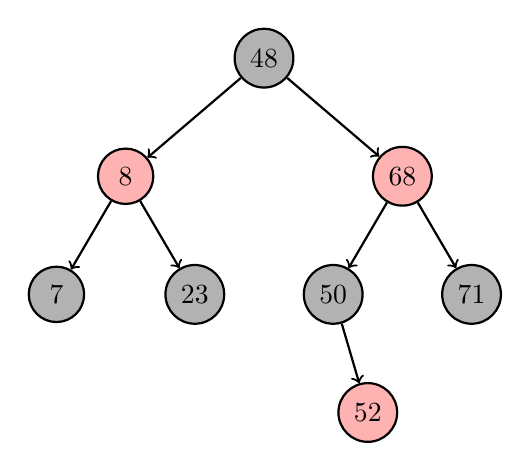
\begin{tikzpicture}[
        redn/.style={fill=red!30},
        blackn/.style={fill=black!30},
        invis/.style={draw=none},
        every node/.style={draw, circle, minimum size=20pt, text centered, thick},
        edge from parent/.style ={draw, ->, thick},
        level 1/.style={sibling distance=100pt},
        level 2/.style={sibling distance=50pt},
        level 3/.style={sibling distance=25pt},
    ]
    \node[blackn](root){48}
    child{node[redn](8){8}
        child{node[blackn](7){7}}
        child{node[blackn](23){23}}
    }
    child{node[redn](68){68}
        child{node[blackn](50){50}
            child{node[invis]{} edge from parent [draw=none]}
            child{node[redn](52){52}}
        }
        child{node[blackn](71){71}}
    }
    ;
    \end{tikzpicture}
    \captionof*{figure}{Richtig Konstruierter RBT}
\end{minipage}
\begin{minipage}[t]{0.5\textwidth}
    \centering
    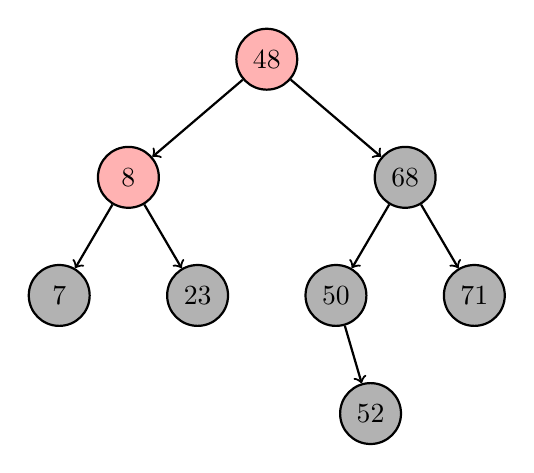
\begin{tikzpicture}[
        redn/.style={fill=red!30},
        blackn/.style={fill=black!30},
        invis/.style={draw=none},
        every node/.style={draw, circle, minimum size=22pt, text centered, thick},
        edge from parent/.style ={draw, ->, thick},
        level 1/.style={sibling distance=100pt},
        level 2/.style={sibling distance=50pt},
        level 3/.style={sibling distance=25pt},
    ]
    \node[redn](root){48}
    child{node[redn](8){8}
        child{node[blackn](7){7}}
        child{node[blackn](23){23}}
    }
    child{node[blackn](68){68}
        child{node[blackn](50){50}
            child{node[invis]{} edge from parent [draw=none]}
            child{node[blackn](52){52}}
        }
        child{node[blackn](71){71}}
    }
    ;
    \end{tikzpicture}
    \captionof*{figure}{Falsch Konstruierter RBT}
\end{minipage}

\textbf{Insertion:}

\begin{algorithm}[H]
    \SetKwFunction{KwRBTree}{RBTree}
    \SetKwFunction{Kwinsert}{insert}
    \SetKwFunction{fixColorsAfterInsertion}{fixColorsAfterInsertion}
    \Cl{\KwRBTree{} \textnormal{(continued)}}{
        \tcp{Complexity: $\Omega(1)$, $O(\log n)$, $\Theta(\log n)$}
        \Fn{\Kwinsert{z}}{
            z.left = sent\;
            z.right = sent\;
            
            x = root; \tcp{Traversal starting from the root}
            px = sent; \tcp{Parent of x, initially sentinel unlike BST}
            
            \While{x $\neq$ sent}{
                px = x\;
                \If{z.key < x.key}{
                    x = x.left\;
                }
                \Else{
                    x = x.right\;
                }
            } \tcp{Traversing the tree until finding the insertion point}
            
            z.parent = px; \tcp{Sets the parent of the node to be inserted}
            
            \If{px == sent}{
                root = z; \tcp{px only sentinel if tree is empty $\rightarrow$ z is root}
            }
            \ElseIf{z.key < px.key}{
                px.left = z; \tcp{Key smaller $\rightarrow$ left child}
            }
            \Else{
                px.right = z; \tcp{Key bigger $\rightarrow$ right child}
            }
            
            z.color = RED; \tcp{Sets color to red, will not necessarily stay red}
            \fixColorsAfterInsertion{z}; \tcp{Fixes colors to maintain RB properties}
        }
    }
\end{algorithm}

Einfügen funktioniert grundlegend gleich zu BST, allerdings wird am Ende die Farbe des neuen Knotens auf rot gesetzt und anschließend die Regeln des RBTs (falls verletzt) wieder hergestellt.

\begin{minipage}[t]{0.5\textwidth}
    \centering
    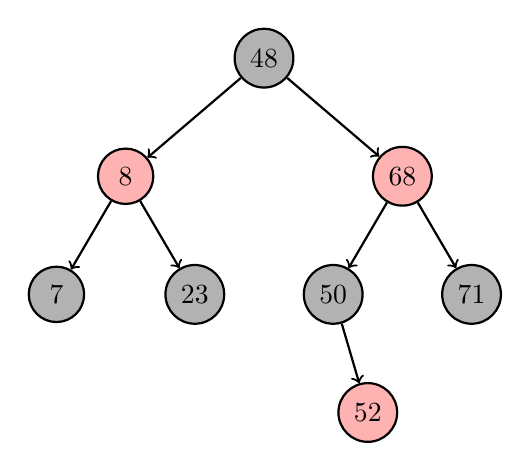
\begin{tikzpicture}[
        redn/.style={fill=red!30},
        blackn/.style={fill=black!30},
        invis/.style={draw=none},
        every node/.style={draw, circle, minimum size=20pt, text centered, thick},
        edge from parent/.style ={draw, ->, thick},
        level 1/.style={sibling distance=100pt},
        level 2/.style={sibling distance=50pt},
        level 3/.style={sibling distance=25pt},
    ]
    \node[blackn](root){48}
    child{node[redn](8){8}
        child{node[blackn](7){7}}
        child{node[blackn](23){23}}
    }
    child{node[redn](68){68}
        child{node[blackn](50){50}
            child{node[invis]{} edge from parent [draw=none]}
            child{node[redn](52){52}}
        }
        child{node[blackn](71){71}}
    }
    ;
    \end{tikzpicture}
    \captionof*{figure}{Before}
\end{minipage}
\begin{minipage}[t]{0.5\textwidth}
    \centering
    \begin{tikzpicture}[
        redn/.style={fill=red!30},
        blackn/.style={fill=black!30},
        invis/.style={draw=none},
        every node/.style={draw, circle, minimum size=20pt, text centered, thick},
        edge from parent/.style ={draw, ->, thick},
        level 1/.style={sibling distance=100pt},
        level 2/.style={sibling distance=50pt},
        level 3/.style={sibling distance=25pt},
    ]
    \node[blackn](root){48}
    child{node[redn](8){8}
        child{node[blackn](7){7}}
        child{node[blackn](23){23}
            child{node[invis]{} edge from parent [draw=none]}
            child{node[redn](37){37}}
        } 
    }
    child{node[redn](68){68}
        child{node[blackn](50){50}
            child{node[invis]{} edge from parent [draw=none]}
            child{node[redn](52){52}}
        }
        child{node[blackn](71){71}}
    }
    ;
    \draw[->, codegreen, very thick] (root) to (8);
    \draw[->, codegreen, very thick] (8) to (23);
    \draw[->, codegreen, very thick] (23) to (37);

    \end{tikzpicture}
    \captionof*{figure}{Insert 37 (No colorfix needed)}
\end{minipage}
\\\vspace{20pt}
\begin{minipage}[t]{0.5\textwidth}
    \centering
    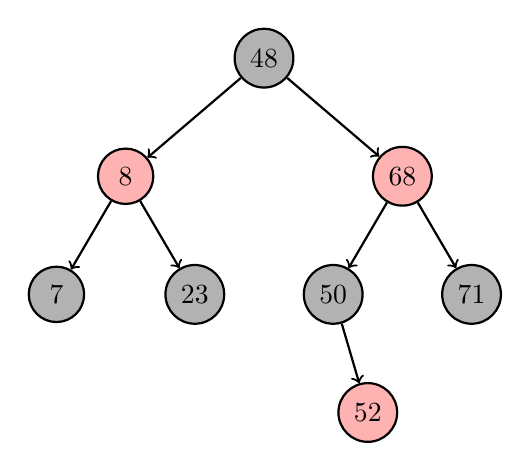
\begin{tikzpicture}[
        redn/.style={fill=red!30},
        blackn/.style={fill=black!30},
        invis/.style={draw=none},
        every node/.style={draw, circle, minimum size=20pt, text centered, thick},
        edge from parent/.style ={draw, ->, thick},
        level 1/.style={sibling distance=100pt},
        level 2/.style={sibling distance=50pt},
        level 3/.style={sibling distance=25pt},
    ]
    \node[blackn](root){48}
    child{node[redn](8){8}
        child{node[blackn](7){7}}
        child{node[blackn](23){23}}
    }
    child{node[redn](68){68}
        child{node[blackn](50){50}
            child{node[invis]{} edge from parent [draw=none]}
            child{node[redn](52){52}}
        }
        child{node[blackn](71){71}}
    }
    ;
    \end{tikzpicture}
    \captionof*{figure}{Before}
\end{minipage}
\begin{minipage}[t]{0.5\textwidth}
    \centering
    \begin{tikzpicture}[
        redn/.style={fill=red!30},
        blackn/.style={fill=black!30},
        invis/.style={draw=none},
        every node/.style={draw, circle, minimum size=20pt, text centered, thick},
        edge from parent/.style ={draw, ->, thick},
        level 1/.style={sibling distance=100pt},
        level 2/.style={sibling distance=50pt},
        level 3/.style={sibling distance=25pt},
    ]
    \node[blackn](root){48}
    child{node[redn](8){8}
        child{node[blackn](7){7}}
        child{node[blackn](23){23}}
    }
    child{node[redn](68){68}
        child{node[blackn](50){50}
            child{node[invis]{} edge from parent [draw=none]}
            child{node[redn](52){52}
                child{node[invis]{} edge from parent [draw=none]}
                child{node[redn](55){55}}
            }
        }
        child{node[blackn](71){71}}
    }
    ;
    \draw[->, codegreen, very thick] (root) to (68);
    \draw[->, codegreen, very thick] (68) to (50);
    \draw[->, codegreen, very thick] (50) to (52);
    \draw[->, codegreen, very thick] (52) to (55);
    \end{tikzpicture}
    \captionof*{figure}{Insert 55 (Colorfix needed)}
\end{minipage}

\newpage
\textbf{Colorfix after Insertion:}

\begin{algorithm}[H]
    \SetKwFunction{KwRBTree}{RBTree}
    \SetKwFunction{rotateLeft}{rotateLeft}
    \SetKwFunction{rotateRight}{rotateRight}
    \SetKwFunction{KwfixColorsAfterInsertion}{fixColorsAfterInsertion}
    \Cl{\KwRBTree{} \textnormal{(continued)}}{
        \tcp{Complexity: $\Omega(1)$, $O(\log n)$, $\Theta(\log n)$}
        \Fn{\KwfixColorsAfterInsertion{z}}{
            \While{z.parent.color == RED}{
                \If{z.parent == z.parent.parent.left}{
                    \tcp{If z's parent is a left child}
                    y = z.parent.parent.right; \tcp{Gets sibling of z's parent}
                    
                    \If{y $\neq$ sent \KwAnd y.color == RED}{
                        \tcp{CASE 1: z's parent is a left child and sibling is red}
                        z.parent.color = BLACK; \tcp{Set z's parent to black}
                        y.color = BLACK; \tcp{Set z's uncle to black}
                        z.parent.parent.color = RED; \tcp{Set z's grandparent to red}
                        z = z.parent.parent; \tcp{Set z to z's grandparent}
                    }
                    \Else{
                        \tcp{CASE 2: z's parent is a left child and sibling is black}
                        \If{z == z.parent.right}{
                            z = z.parent; \tcp{If z is a right child, set z to parent}
                            \rotateLeft{z}; \tcp{Rotate new z to left}
                        }
                        z.parent.color = BLACK; \tcp{Set z's parent to black}
                        z.parent.parent.color = RED; \tcp{Set z's grandparent to red}
                        \rotateRight{z.parent.parent}; \tcp{Rotate z's grandparent to right}
                    }
                }
                \Else{
                    \tcp{If z's parent is a right child (Same as above but exchanged)}
                    y = z.parent.parent.left\;
                    \If{y $\neq$ sent \KwAnd y.color == RED}{
                        \tcp{CASE 3: z's parent is a right child and sibling is red}
                        z.parent.color = BLACK\;
                        y.color = BLACK\;
                        z.parent.parent.color = RED\;
                        z = z.parent.parent\;
                    }
                    \Else{
                        \tcp{CASE 4: z's parent is a right child and sibling is black}
                        \If{z == z.parent.left}{
                            z = z.parent\;
                            \rotateRight{z}\;
                        }
                        z.parent.color = BLACK\;
                        z.parent.parent.color = RED\;
                        \rotateLeft{z.parent.parent}\;
                    }
                }
            }
            root.color = BLACK; \tcp{Set root to black, as it always should be}
        }
    }
\end{algorithm}

\begin{minipage}[t]{0.5\textwidth}
    \centering
    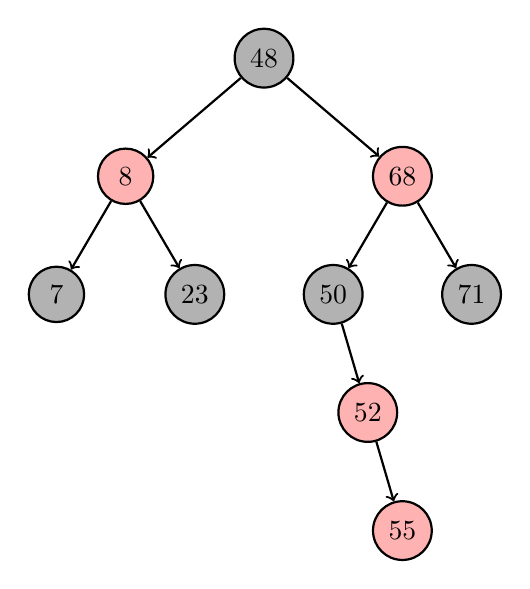
\begin{tikzpicture}[
        redn/.style={fill=red!30},
        blackn/.style={fill=black!30},
        invis/.style={draw=none},
        every node/.style={draw, circle, minimum size=20pt, text centered, thick},
        edge from parent/.style ={draw, ->, thick},
        level 1/.style={sibling distance=100pt},
        level 2/.style={sibling distance=50pt},
        level 3/.style={sibling distance=25pt},
    ]
    \node[blackn](root){48}
    child{node[redn](8){8}
        child{node[blackn](7){7}}
        child{node[blackn](23){23}}
    }
    child{node[redn](68){68}
        child{node[blackn](50){50}
            child{node[invis]{} edge from parent [draw=none]}
            child{node[redn](52){52}
                child{node[invis]{} edge from parent [draw=none]}
                child{node[redn](55){55}}
            }
        }
        child{node[blackn](71){71}}
    }
    ;
    \end{tikzpicture}
    \captionof*{figure}{Fix needed at 55}
\end{minipage}
\begin{minipage}[t]{0.5\textwidth}
    \centering
    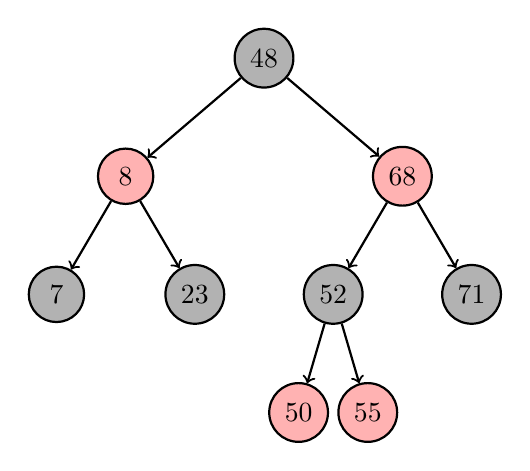
\begin{tikzpicture}[
        redn/.style={fill=red!30},
        blackn/.style={fill=black!30},
        invis/.style={draw=none},
        every node/.style={draw, circle, minimum size=20pt, text centered, thick},
        edge from parent/.style ={draw, ->, thick},
        level 1/.style={sibling distance=100pt},
        level 2/.style={sibling distance=50pt},
        level 3/.style={sibling distance=25pt},
    ]
    \node[blackn](root){48}
    child{node[redn](8){8}
        child{node[blackn](7){7}}
        child{node[blackn](23){23}}
    }
    child{node[redn](68){68}
        child{node[blackn](52){52}
            child{node[redn](50){50}}
            child{node[redn](55){55}}
        }
        child{node[blackn](71){71}}
    }
    ;
    \end{tikzpicture}
    \captionof*{figure}{Fixed (Case 4)}
\end{minipage}

\textbf{Rotation:}

Zum Wiederherstellen der RBT-Regeln muss der Baum an bestimmten Knoten rotiert werden.

\begin{algorithm}[H]
    \SetKwFunction{KwRBTree}{RBTree}
    \SetKwFunction{KwrotateLeft}{rotateLeft}
    \SetKwFunction{KwrotateRight}{rotateRight}
    \Cl{\KwRBTree{} \textnormal{(continued)}}{
        \tcp{Complexity: $O(1)$}
        \Fn{\KwrotateLeft{x}}{
            y = x.right\;
            x.right = y.left; \tcp{Set x's right child to y's left child}
            
            \If{y.left $\neq$ sent}{
                y.left.parent = x; \tcp{Set y's left child's parent to x}
            }
            y.parent = x.parent; \tcp{Set y's parent to x's parent}
            
            \If{x.parent == sent}{
                root = y; \tcp{If x is the root, set y to be the root}
            }
            \ElseIf{x == x.parent.left}{
                x.parent.left = y; \tcp{If x is a left child, set x's parent's left child to y}
            }
            \Else{
                x.parent.right = y; \tcp{If x is a right child, set x's parent's right child to y}
            }
            y.left = x; \tcp{Set y's left child to x}
            x.parent = y; \tcp{Set x's parent to y}
        }
                
        \tcp{Complexity: $O(1)$}
        \Fn{\KwrotateRight{x}}{
            y = x.left\;
            x.left = y.right\;
            
            \If{y.right $\neq$ sent}{
                y.right.parent = x\;
            }
            y.parent = x.parent\;
            
            \If{x.parent == sent}{
                root = y\;
            }
            \ElseIf{x == x.parent.right}{
                x.parent.right = y\;
            }
            \Else{
                x.parent.left = y\;
            }
            y.right = x\;
            x.parent = y\;
        }
    }
\end{algorithm}

\begin{minipage}[t]{\textwidth}
    \centering
    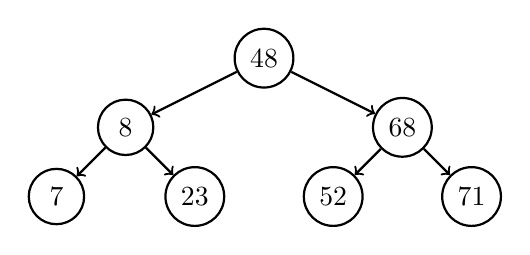
\begin{tikzpicture}[
        level distance=25pt,
        invis/.style={draw=none},
        every node/.style={draw, circle, minimum size=20pt, text centered, thick},
        edge from parent/.style ={draw, ->, thick},
        level 1/.style={sibling distance=100pt},
        level 2/.style={sibling distance=50pt},
        level 3/.style={sibling distance=25pt},
    ]
    \node[](root){48}
    child{node[](8){8}
        child{node[](7){7}}
        child{node[](23){23}}
    }
    child{node[](68){68}
        child{node[](52){52}}
        child{node[](71){71}}
    }
    ;
    \end{tikzpicture}
    \captionof*{figure}{Before}
\end{minipage}
\begin{minipage}[t]{0.5\textwidth}
    \centering
    \begin{tikzpicture}[
        level distance=25pt,
        invis/.style={draw=none},
        every node/.style={draw, circle, minimum size=20pt, text centered, thick},
        edge from parent/.style ={draw, ->, thick},
        level 1/.style={sibling distance=100pt},
        level 2/.style={sibling distance=50pt},
        level 3/.style={sibling distance=25pt},
    ]
    \node[](root){48}
    child{node[](8){8}
        child{node[](7){7}}
        child{node[](23){23}}
    }
    child{node[](68){68}
        child{node[](52){52}}
        child{node[](71){71}}
    }
    ;
    \draw[->, codegreen, thick, bend right] (root) to (8);
    \draw[->, codegreen, very thick] (52) to (23);
    \draw[->, codegreen, thick, bend right] (71) to (68);
    \draw[->, codegreen, thick, bend right] (68) to (root);
    \end{tikzpicture}
    \captionof*{figure}{rotateLeft(root)}
\end{minipage}
\begin{minipage}[t]{0.5\textwidth}
    \centering
    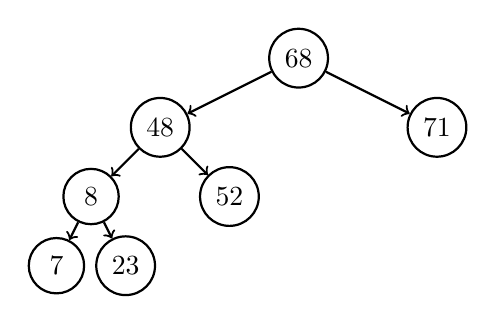
\begin{tikzpicture}[
        level distance=25pt,
        invis/.style={draw=none},
        every node/.style={draw, circle, minimum size=20pt, text centered, thick},
        edge from parent/.style ={draw, ->, thick},
        level 1/.style={sibling distance=100pt},
        level 2/.style={sibling distance=50pt},
        level 3/.style={sibling distance=25pt},
    ]
    \node[](root){68}
    child{node[](48){48}
        child{node[](8){8}
            child{node[](7){7}}
            child{node[](23){23}}
        }
        child{node[](52){52}}
    }
    child{node[](71){71}}
    ;
    \end{tikzpicture}
    \captionof*{figure}{rotateLeft(root) result}
\end{minipage}
\begin{minipage}[t]{0.5\textwidth}
    \centering
    \begin{tikzpicture}[
        level distance=25pt,
        invis/.style={draw=none},
        every node/.style={draw, circle, minimum size=20pt, text centered, thick},
        edge from parent/.style ={draw, ->, thick},
        level 1/.style={sibling distance=100pt},
        level 2/.style={sibling distance=50pt},
        level 3/.style={sibling distance=25pt},
    ]
    \node[](root){48}
    child{node[](8){8}
        child{node[](7){7}}
        child{node[](23){23}}
    }
    child{node[](68){68}
        child{node[](52){52}}
        child{node[](71){71}}
    }
    ;
    \draw[->, codegreen, thick, bend left] (root) to (68);
    \draw[->, codegreen, very thick] (23) to (52);
    \draw[->, codegreen, thick, bend left] (7) to (8);
    \draw[->, codegreen, thick, bend left] (8) to (root);
    \end{tikzpicture}
    \captionof*{figure}{rotateRight(root)}
\end{minipage}
\begin{minipage}[t]{0.5\textwidth}
    \centering
    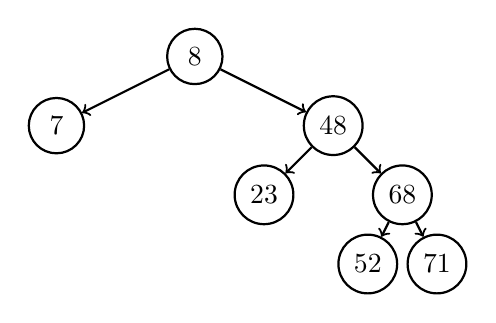
\begin{tikzpicture}[
        level distance=25pt,
        invis/.style={draw=none},
        every node/.style={draw, circle, minimum size=20pt, text centered, thick},
        edge from parent/.style ={draw, ->, thick},
        level 1/.style={sibling distance=100pt},
        level 2/.style={sibling distance=50pt},
        level 3/.style={sibling distance=25pt},
    ]
    \node[](root){8}
    child{node[](7){7}}
    child{node[](48){48}
        child{node[](23){23}}
        child{node[](68){68}
            child{node[](52){52}}
            child{node[](71){71}}
        }
    }
    ;
    \end{tikzpicture}
    \captionof*{figure}{rotateRight(root) result}
\end{minipage}

\newpage
\textbf{Deletion:}

\begin{algorithm}[H]
    \SetKwFunction{KwRBTree}{RBTree}
    \SetKwFunction{Kwdelete}{delete}
    \SetKwFunction{fixColorsAfterDeletion}{fixColorsAfterDeletion}
    \SetKwFunction{transplant}{transplant}
    \Cl{\KwRBTree{} \textnormal{(continued)}}{
        \tcp{Complexity: $\Omega(1)$, $O(\log n)$, $\Theta(\log n)$}
        \Fn{\Kwdelete{z}}{
            a = z.parent; \tcp{a represent node with black depth imbalance}
            dbh = 0; \tcp{delta black height, -1 for right, 1 for left leaning}
            
            \If{z.left == sent \KwAnd z.right == sent}{
                \tcp{CASE 1: z is a leaf}
                \If{z.color == BLACK \KwAnd z $\neq$ root}{
                    \If{z == z.parent.left}{
                        dbh = -1; \tcp{Set delta black height to -1}
                    }
                    \Else{
                        dbh = 1; \tcp{Set delta black height to 1}
                    }
                }
                \transplant{z, sent}; \tcp{Transplant sentinel to z's parent}
            }
            \ElseIf{z.left == sent}{
                \tcp{CASE 2: z only has a right child}
                y = z.right\;
                \transplant{z, z.right}\;
                y.color = z.color\;
            }
            \ElseIf{z.right == sent}{
                \tcp{CASE 3: z only has a left child}
                y = z.left\;
                \transplant{z, z.left}\;
                y.color = z.color\;
            }
            \Else{
                \tcp{CASE 4: z has two children}
                y = z.right\;
                a = y\;
                wentLeft = \KwFalse\;
                
                \While{y.left $\neq$ sent}{
                    \tcp{find next biggest Node}
                    a = y\;
                    y = y.left\;
                    wentLeft = \KwTrue\;
                }
                
                \If{y.parent $\neq$ z}{
                    \tcp{If next biggest element is not child of z}
                    \transplant{y, y.right}\;
                    y.right = z.right\;
                    y.right.parent = y\;
                }
                \transplant{z, y}\;
                y.left = z.left\;
                y.left.parent = y\;
                
                \If{y.color == BLACK}{
                    \If{wentLeft}{
                        dbh = -1; \tcp{Tree imbalanced depending on y location}
                    }
                    \Else{
                        dbh = 1\;
                    }
                }
                y.color = z.color\;
            }
            
            \If{dbh $\neq$ 0}{
                \fixColorsAfterDeletion{a, dbh}; \tcp{If black height imbalance}
            }
        }
    }
\end{algorithm}

\begin{minipage}[t]{1\textwidth}
    \centering
    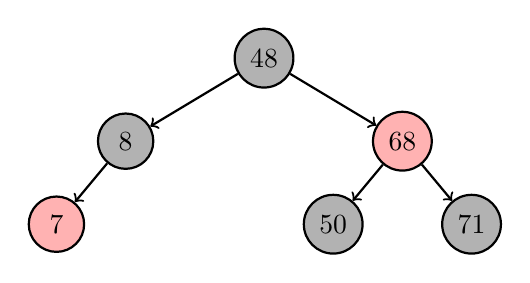
\begin{tikzpicture}[
        redn/.style={fill=red!30},
        blackn/.style={fill=black!30},
        invis/.style={draw=none},
        every node/.style={draw, circle, minimum size=20pt, text centered, thick},
        edge from parent/.style ={draw, ->, thick},
        level 1/.style={sibling distance=100pt},
        level 2/.style={sibling distance=50pt},
        level 3/.style={sibling distance=25pt},
        level distance=30pt,
    ]
    \node[blackn](root){48}
    child{node[blackn](8){8}
        child{node[redn](7){7}}
        child{node[invis]{} edge from parent [draw=none]}
    }
    child{node[redn](68){68}
        child{node[blackn](50){50}}
        child{node[blackn](71){71}}
    }
    ;
    \end{tikzpicture}
    \captionof*{figure}{Before}
\end{minipage}
\begin{minipage}[t]{0.5\textwidth}
    \centering
    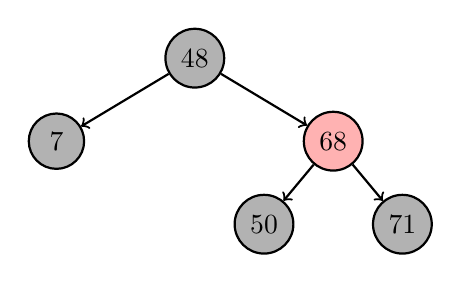
\begin{tikzpicture}[
        redn/.style={fill=red!30},
        blackn/.style={fill=black!30},
        invis/.style={draw=none},
        every node/.style={draw, circle, minimum size=20pt, text centered, thick},
        edge from parent/.style ={draw, ->, thick},
        level 1/.style={sibling distance=100pt},
        level 2/.style={sibling distance=50pt},
        level 3/.style={sibling distance=25pt},
        level distance=30pt,
    ]
    \node[blackn](root){48}
    child{node[blackn](7){7}}
    child{node[redn](68){68}
        child{node[blackn](50){50}}
        child{node[blackn](71){71}}
    }
    ;
    \end{tikzpicture}
    \captionof*{figure}{Delete 8 (No colorfix needed, Case 3)}
\end{minipage}
\begin{minipage}[t]{0.5\textwidth}
    \centering
    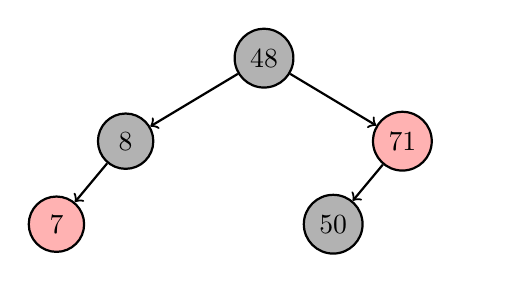
\begin{tikzpicture}[
        redn/.style={fill=red!30},
        blackn/.style={fill=black!30},
        invis/.style={draw=none},
        every node/.style={draw, circle, minimum size=20pt, text centered, thick},
        edge from parent/.style ={draw, ->, thick},
        level 1/.style={sibling distance=100pt},
        level 2/.style={sibling distance=50pt},
        level 3/.style={sibling distance=25pt},
        level distance=30pt,
    ]
    \node[blackn](root){48}
    child{node[blackn](8){8}
        child{node[redn](7){7}}
        child{node[invis]{} edge from parent [draw=none]}
    }
    child{node[redn](71){71}
        child{node[blackn](50){50}}
        child{node[invis]{} edge from parent [draw=none]}
    }
    ;
    \end{tikzpicture}
    \captionof*{figure}{Delete 68 (Colorfix needed, Case 4, $dbh = 1$, skewed left)}
\end{minipage}

\newpage
\textbf{Colorfix after Deletion:}

\begin{algorithm}[H]
    \SetKwFunction{KwRBTree}{RBTree}
    \SetKwFunction{fixColorsAfterDeletion}{fixColorsAfterDeletion}
    \SetKwFunction{rotateLeft}{rotateLeft}
    \SetKwFunction{rotateRight}{rotateRight}
    \SetKwFunction{transplant}{transplant}
    \Cl{\KwRBTree{} \textnormal{(continued)}}{
        \tcp{Complexity: $\Omega(1)$, $O(\log n)$, $\Theta(\log n)$}
        \Fn{\fixColorsAfterDeletion{a, dbh}}{
            \If{dbh == -1}{
                \tcp{Extra black node on the right}
                x = a.left\;
                b = a.right\;
                c = b.left; \tcp{Left child of right child of a}
                d = b.right; \tcp{Right child of right child of a}
                
                \tcp{Fixed: Replaced all null checks with sent}
                \If{x $\neq$ sent \KwAnd x.color == RED}{
                    x.color = BLACK; \tcp{Easy case: x is red}
                }
                \ElseIf{a.color == BLACK \KwAnd b.color == RED}{
                    \tcp{Case 1: a black, b red}
                    \rotateLeft{a}\;
                    a.color = RED\;
                    b.color = BLACK\;
                    \fixColorsAfterDeletion{a, dbh}\;
                }
                \ElseIf{a.color == RED \KwAnd b.color == BLACK \KwAnd (c == sent \KwOr c.color == BLACK) \KwAnd (d == sent \KwOr d.color == BLACK)}{
                    \tcp{Case 2a: a red, b black, c and d black}
                    a.color = BLACK\;
                    b.color = RED\;
                }
                \ElseIf{a.color == BLACK \KwAnd b.color == BLACK \KwAnd (c == sent \KwOr c.color == BLACK) \KwAnd (d == sent \KwOr d.color == BLACK)}{
                    \tcp{Case 2b: a black, b black, c and d black}
                    b.color = RED\;
                    \If{a == a.parent.left}{
                        dbh = 1\;
                    }
                    \ElseIf{a == a.parent.right}{
                        dbh = -1\;
                    }
                    \Else{
                        dbh = 0\;
                    }
                    \fixColorsAfterDeletion{a.parent, dbh}\;
                }
                \ElseIf{b.color == BLACK \KwAnd c $\neq$ sent \KwAnd c.color == RED \KwAnd (d == sent \KwOr d.color == BLACK)}{
                    \tcp{Case 3: a either, b black, c red, d black}
                    \rotateRight{b}\;
                    c.color = BLACK\;
                    \fixColorsAfterDeletion{a, dbh}\;
                }
                \ElseIf{b.color == BLACK \KwAnd d $\neq$ sent \KwAnd d.color == RED}{
                    \tcp{Case 4: a either, b black, c either, d red}
                    \rotateLeft{a}\;
                    b.color = a.color\;
                    a.color = BLACK\;
                    d.color = BLACK\;
                }
            }
            \tcp{Conitinued on next Page:}
        }
    }
\end{algorithm}

\begin{algorithm}[H]
    \setcounter{AlgoLine}{44}
    \SetKwFunction{KwRBTree}{RBTree}
    \SetKwFunction{fixColorsAfterDeletion}{fixColorsAfterDeletion}
    \SetKwFunction{rotateLeft}{rotateLeft}
    \SetKwFunction{rotateRight}{rotateRight}
    \SetKwFunction{transplant}{transplant}
    \Cl{\KwRBTree{} \textnormal{(continued)}}{
        \Fn{\fixColorsAfterDeletion{a, dbh} (continued)}{
            \Else{
                \tcp{Extra black node on the left (Same as above but with right and left exchanged)}
                x = a.right\;
                b = a.left\;
                c = b.right; \tcp{Right child of left child of a}
                d = b.left; \tcp{Left child of left child of a}
                
                \If{x $\neq$ sent \KwAnd x.color == RED}{
                    x.color = BLACK\;
                }
                \ElseIf{a.color == BLACK \KwAnd b.color == RED}{
                    \rotateRight{a}\;
                    a.color = RED\;
                    b.color = BLACK\;
                    \fixColorsAfterDeletion{a, dbh}\;
                }
                \ElseIf{a.color == RED \KwAnd b.color == BLACK \KwAnd (c == sent \KwOr c.color == BLACK) \KwAnd (d == sent \KwOr d.color == BLACK)}{
                    a.color = BLACK\;
                    b.color = RED\;
                }
                \ElseIf{a.color == BLACK \KwAnd b.color == BLACK \KwAnd (c == sent \KwOr c.color == BLACK) \KwAnd (d == sent \KwOr d.color == BLACK)}{
                    b.color = RED\;
                    \If{a == a.parent.right}{
                        dbh = 1\;
                    }
                    \ElseIf{a == a.parent.left}{
                        dbh = -1\;
                    }
                    \Else{
                        dbh = 0\;
                    }
                    \fixColorsAfterDeletion{a.parent, dbh}\;
                }
                \ElseIf{b.color == BLACK \KwAnd c $\neq$ sent \KwAnd c.color == RED \KwAnd (d == sent \KwOr d.color == BLACK)}{
                    \rotateLeft{b}\;
                    c.color = BLACK\;
                    \fixColorsAfterDeletion{a, dbh}\;
                }
                \ElseIf{b.color == BLACK \KwAnd d $\neq$ sent \KwAnd d.color == RED}{
                    \rotateRight{a}\;
                    b.color = a.color\;
                    a.color = BLACK\;
                    d.color = BLACK\;
                }
            }
            \tcp{All cases except 2b mean end of the method in this or the next instance. 2b can go on tho.}
        }
    }
\end{algorithm}

\begin{minipage}[t]{0.5\textwidth}
    \centering
    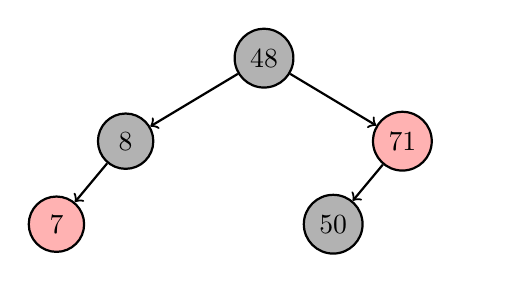
\begin{tikzpicture}[
        redn/.style={fill=red!30},
        blackn/.style={fill=black!30},
        invis/.style={draw=none},
        every node/.style={draw, circle, minimum size=20pt, text centered, thick},
        edge from parent/.style ={draw, ->, thick},
        level 1/.style={sibling distance=100pt},
        level 2/.style={sibling distance=50pt},
        level 3/.style={sibling distance=25pt},
        level distance=30pt,
    ]
    \node[blackn](root){48}
    child{node[blackn](8){8}
        child{node[redn](7){7}}
        child{node[invis]{} edge from parent [draw=none]}
    }
    child{node[redn](71){71}
        child{node[blackn](50){50}}
        child{node[invis]{} edge from parent [draw=none]}
    }
    ;
    \end{tikzpicture}
    \captionof*{figure}{Before fix}
\end{minipage}
\begin{minipage}[t]{0.5\textwidth}
    \centering
    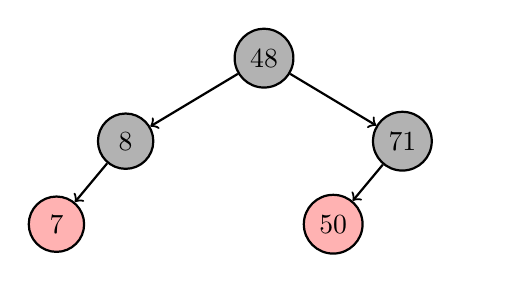
\begin{tikzpicture}[
        redn/.style={fill=red!30},
        blackn/.style={fill=black!30},
        invis/.style={draw=none},
        every node/.style={draw, circle, minimum size=20pt, text centered, thick},
        edge from parent/.style ={draw, ->, thick},
        level 1/.style={sibling distance=100pt},
        level 2/.style={sibling distance=50pt},
        level 3/.style={sibling distance=25pt},
        level distance=30pt,
    ]
    \node[blackn](root){48}
    child{node[blackn](8){8}
        child{node[redn](7){7}}
        child{node[invis]{} edge from parent [draw=none]}
    }
    child{node[blackn](71){71}
        child{node[redn](50){50}}
        child{node[invis]{} edge from parent [draw=none]}
    }
    ;
    \end{tikzpicture}
    \captionof*{figure}{Fixed (Case 2a)}
\end{minipage}

\newpage
\textbf{Transplant:}

\begin{algorithm}[H]
    \SetKwFunction{KwRBTree}{RBTree}
    \SetKwFunction{transplant}{transplant}
    \Cl{\KwRBTree{} \textnormal{(continued)}}{
        \tcp{Complexity: $O(1)$}
        \Fn{\transplant{u, v}}{
            \tcp{Transplants v to the position of u}
            \If{u.parent == sent}{
                root = v; \tcp{If u is the root, v becomes the new root}
            }
            \ElseIf{u == u.parent.left}{
                u.parent.left = v; \tcp{If u is a left child, v becomes a left child}
            }
            \Else{
                u.parent.right = v; \tcp{If u is a right child, v becomes a right child}
            }
            
            \If{v $\neq$ sent}{
                v.parent = u.parent; \tcp{If v is not null, v becomes a child of u's parent}
            }
        }
    }
\end{algorithm}

Eine schöne interaktive Visualisierung von RBTs kann man \href{https://www.cs.usfca.edu/~galles/visualization/RedBlack.html}{hier} finden.

\includepdf[pages={15,19-20,133-}, pagecommand={},nup=2x2, frame=true, scale=0.9]{../VL_Folien/04AdvancedDataStructures.pdf}
\subsection{AVL Trees}
Ein \textbf{A}delson-\textbf{V}elsky \textbf{L}andis Tree ist ein BST, der sich selbst balanziert um eine Höhe von $h = \log n$ zu garantieren. Er wird so definiert, \textbf{dass die Höhendifferenz von zwei Teilbäumen unter einem Knoten jeweils maximal $1$ ist}.\\
Im Vergleich zu RBT ist der AVLT in der Höhe strikter. So ist die maximale Höhe im AVL $h = 1.44 \cdot \log (n + 2)$, während er im RBT nur $2 \cdot \log n$. So haben AVLTs zwar die bessere Effizienz in Suchvorgängen, jedoch benötigen sie beim Insert oder Delete meist mehr Rotationen. Demnach bieten sich AVLTs eher bei Fällen an, wo mehr Suchvorgänge stattfinden im Vergleich zu den Insert/Delete Vorgängen. Muss der Baum oft modifiziert werden so bietet sich ein RBT besser an.\\ Die minimale Anzahl an Knoten in einem AVL-Tree mit Höhe h ergibt sich durch die rekursive Fibonaci-Gleichung: $N(h) = N(h - 1) + N(h - 2) + 1$ mit $N(0) = 1$ und $N(1) = 2$. (Root hat Maximalhöhe, Blätter sind h = 0)\\

\textbf{Definition:}

\begin{algorithm}[H]
    \SetKwFunction{KwAVLTree}{AVLTree}
    \SetKwFunction{KwAVLNode}{AVLNode}
    \SetKwFunction{kwheight}{height}
    \SetKwFunction{updateHeight}{updateHeight}
    \SetKwFunction{getBalance}{getBalance}
    \Cl{\KwAVLNode{}}{
        key\;
        height\;
        left = \KwNil\;
        right = \KwNil\;
        \Con{\KwAVLNode{k}}{
            key = k\;
            height = 1\;
        }
    }
    \Cl{\KwAVLTree{}}{
        root = \KwNil\;
        \tcp{Complexity: O(1)}
        \Fn{\kwheight{n}}{
            \If{n $==$ \KwNil}{
                \KwRet 0;
            }
            \KwRet n.height\;
        }
        \tcp{Complexity: O(1)}
        \Fn{\updateHeight{n}}{
            n.height = 1 $+$ $\max$(\kwheight{n.left}, \kwheight{n.right})\;
        }
        \tcp{Complexity: O(1)}
        \Fn{\getBalance{n}}{
            \If{n $==$ \KwNil}{
                \KwRet 0\;
            }
            \KwRet \kwheight{n.right} $-$ \kwheight{n.left}\;
        }
    }
\end{algorithm}


Visuell gleich zu einem Best-Case ausgewogenen BST. \\
\begin{minipage}[t]{0.5\textwidth}
    \centering
    \begin{tikzpicture}[
        invis/.style={draw=none},
        every node/.style={draw, circle, minimum size=20pt, text centered, thick},
        edge from parent/.style ={draw, ->, thick},
        level 1/.style={sibling distance=100pt},
        level 2/.style={sibling distance=50pt},
        level 3/.style={sibling distance=25pt},
        level distance=30pt,
    ]
    \node[](root){17}
    child{node[](9){9}
        child{node[invis]{} edge from parent [draw=none]}
        child{node[](11){11}}
    }
    child{node[](23){23}
        child{node[](22){22}}
        child{node[](32){32}}
    }
    ;
    \node[left= 0pt of 11, invis]{0};
    \node[left= 0pt of 22, invis]{0};
    \node[left= 0pt of 9, invis]{+1};
    \node[above= 0pt of root, invis]{0};
    \node[right= 0pt of 23, invis]{0};
    \node[right= 0pt of 32, invis]{0};

    \end{tikzpicture}
    \captionof*{figure}{Balanced Tree}
\end{minipage}
\begin{minipage}[t]{0.5\textwidth}
    \centering
    \begin{tikzpicture}[
        invis/.style={draw=none},
        every node/.style={draw, circle, minimum size=20pt, text centered, thick},
        edge from parent/.style ={draw, ->, thick},
        level 1/.style={sibling distance=100pt},
        level 2/.style={sibling distance=50pt},
        level 3/.style={sibling distance=25pt},
        level distance=30pt,
    ]
    \node[](root){23}
    child{node[](17){17}
        child{node[](9){9}
            child{node[invis]{} edge from parent [draw=none]}
            child{node[](11){11}}
        }
        child{node[](22){22}}
    }
    child{node[](32){32}}
    ;
    \node[left= 0pt of 11, invis]{0};
    \node[left= 0pt of 22, invis]{0};
    \node[left= 0pt of 9, invis]{+1};
    \node[left= 0pt of 17, invis]{-1};
    \node[above= 0pt of root, invis, red]{-2};
    \node[right= 0pt of 32, invis]{0};

    \end{tikzpicture}
    \captionof*{figure}{Unbalanced Tree}
\end{minipage}

\newpage
\textbf{Rotation:}

\begin{algorithm}[H]
    \SetKwFunction{KwAVLTree}{AVLTree}
    \SetKwFunction{rotateLeft}{rotateLeft}
    \SetKwFunction{rotateRight}{rotateRight}
    \SetKwFunction{updateHeight}{updateHeight}
    \Cl{\KwAVLTree{} \textnormal{(continued)}}{
        \tcp{Complexity: O(1)}
        \Fn{\rotateLeft{x}}{
            y = x.right\;
            z = y.left\;
            y.left = x\;
            x.right = z\;
            \updateHeight{x}\;
            \updateHeight{y}\;
            \KwRet y\;
        }
        \tcp{Complexity: O(1)}
        \Fn{\rotateRight{x}}{
            y = x.left\;
            z = y.right\;
            y.right = x\;
            x.left = z\;
            \updateHeight{x}\;
            \updateHeight{y}\;
            \KwRet y\;
        }
    }
\end{algorithm}

Während die Function ein wenig abgeändert ist, ist das Endergebnis bei richtiger Anwendung (nicht inPlace) gleich.

\textbf{Insertion:}

\begin{algorithm}[H]
    \SetKwFunction{KwAVLTree}{AVLTree}
    \SetKwFunction{Kwinsert}{insert}
    \SetKwFunction{fixBalance}{fixBalance}
    \Cl{\KwAVLTree{} \textnormal{(continued)}}{
        \tcp{Complexity: O(h) = O(log(n))}
        \Fn{\Kwinsert{partRoot, key}}{
            \If{partRoot $==$ \KwNil}{
                \KwRet \text{new } \KwAVLNode{key}; \tcp{Found insertion point}
            }
            \ElseIf{key $<$ partRoot.key}{
                partRoot.left = \Kwinsert{partRoot.left, key}\;
            }
            \ElseIf{key $>$ partRoot.key}{
                partRoot.right = \Kwinsert{partRoot.right, key}\;
            }
            \Else{
                \KwRet \KwError; \tcp{Duplicate node}
            }
            \KwRet \fixBalance{partRoot}; \tcp{Rebalance every node above the inserted node}
        }
    }
\end{algorithm}

Funktioniert prinzipiell gleich zu den anderen Trees, aber ist nicht in-place und muss zusätzlich noch alle subtrees balanzieren.

\newpage
\textbf{Deletion:}

\begin{algorithm}[H]
    \SetKwFunction{KwAVLTree}{AVLTree}
    \SetKwFunction{Kwdelete}{delete}
    \SetKwFunction{fixBalance}{fixBalance}
    \Cl{\KwAVLTree{} \textnormal{(continued)}}{
        \tcp{Complexity: O(h) = O(log(n))}
        \Fn{\Kwdelete{node, key}}{
            \If{node $==$ \KwNil}{
                \KwRet node; \tcp{Node not found}
            }
            \ElseIf{key $<$ node.key}{
                node.left = \Kwdelete{node.left, key}\;
            }
            \ElseIf{key $>$ node.key}{
                node.right = \Kwdelete{node.right, key}\;
            }
            \Else{
                \tcp{Node found -> Commence deletion}
                \If{node.left $==$ \KwNil \KwOr node.right $==$ \KwNil}{
                    \If{node.left $==$ \KwNil}{
                        node = node.right\;
                    }
                    \Else{
                        node = node.left\;
                    }
                }
                \Else{
                    \tcp{If complete node}
                    next = node.right\;
                    \While{next.left $\neq$ \KwNil}{
                        next = next.left\;
                    }
                    node.key = next.key\;
                    node.right = \Kwdelete{node.right, next.key}\;
                }
            }
            \KwRet \fixBalance{node}; \tcp{Rebalance every node above the deleted node}
        }
    }
\end{algorithm}

Wie bei rotate und insert, prinzipiell gleich zu den anderen Trees, aber ist nicht in-place und muss zusächlich alle subtrees balanzieren.

\newpage
\textbf{Balancefix:}

\begin{algorithm}[H]
    \SetKwFunction{KwAVLTree}{AVLTree}
    \SetKwFunction{fixBalance}{fixBalance}
    \SetKwFunction{updateHeight}{updateHeight}
    \SetKwFunction{getBalance}{getBalance}
    \SetKwFunction{rotateLeft}{rotateLeft}
    \SetKwFunction{rotateRight}{rotateRight}
    \SetKwFunction{Kwheight}{height}
    \Cl{\KwAVLTree{} \textnormal{(continued)}}{
        \tcp{Complexity: O(1)}
        \Fn{\fixBalance{z}}{
            \tcp{Fixed: Handle null to prevent crash when deleting leaf nodes}
            \If{z $==$ \KwNil}{
                \KwRet \KwNil\;
            }
            \updateHeight{z}\;
            balance = \getBalance{z}\;
            \If{balance $>$ 1}{
                \tcp{If right heavy}
                \If{\Kwheight{z.right.right} $>$ \Kwheight{z.right.left}}{
                    z = \rotateLeft{z}\;
                }
                \Else{
                    z.right = \rotateRight{z.right}\;
                    z = \rotateLeft{z}\;
                }
            }
            \ElseIf{balance $<$ -1}{
                \tcp{If left heavy}
                \If{\Kwheight{z.left.left} $>$ \Kwheight{z.left.right}}{
                    z = \rotateRight{z}\;
                }
                \Else{
                    z.left = \rotateLeft{z.left}\;
                    z = \rotateRight{z}\;
                }
            }
            \KwRet z\;
        }
    }
\end{algorithm}

\begin{minipage}[t]{0.5\textwidth}
    \centering
    \begin{tikzpicture}[
        invis/.style={draw=none},
        every node/.style={draw, circle, minimum size=20pt, text centered, thick},
        edge from parent/.style ={draw, ->, thick},
        level 1/.style={sibling distance=100pt},
        level 2/.style={sibling distance=50pt},
        level 3/.style={sibling distance=25pt},
        level distance=30pt,
    ]
    \node[](root){23}
    child{node[](17){17}
        child{node[](9){9}
            child{node[invis]{} edge from parent [draw=none]}
            child{node[](11){11}}
        }
        child{node[](22){22}}
    }
    child{node[](32){32}}
    ;
    \node[left= 0pt of 11, invis]{0};
    \node[left= 0pt of 22, invis]{0};
    \node[left= 0pt of 9, invis]{+1};
    \node[left= 0pt of 17, invis]{-1};
    \node[above= 0pt of root, invis, red]{-2};
    \node[right= 0pt of 32, invis]{0};

    \end{tikzpicture}
    \captionof*{figure}{Unbalanced Tree after insert of 11}
\end{minipage}
\begin{minipage}[t]{0.5\textwidth}
    \centering
    \begin{tikzpicture}[
        invis/.style={draw=none},
        every node/.style={draw, circle, minimum size=20pt, text centered, thick},
        edge from parent/.style ={draw, ->, thick},
        level 1/.style={sibling distance=100pt},
        level 2/.style={sibling distance=50pt},
        level 3/.style={sibling distance=25pt},
        level distance=30pt,
    ]
    \node[](root){17}
    child{node[](9){9}
        child{node[invis]{} edge from parent [draw=none]}
        child{node[](11){11}}
    }
    child{node[](23){23}
        child{node[](22){22}}
        child{node[](32){32}}
    }
    ;
    \node[left= 0pt of 11, invis]{0};
    \node[left= 0pt of 22, invis]{0};
    \node[left= 0pt of 9, invis]{+1};
    \node[above= 0pt of root, invis]{0};
    \node[right= 0pt of 23, invis]{0};
    \node[right= 0pt of 32, invis]{0};

    \end{tikzpicture}
    \captionof*{figure}{Balanced Tree after fixup}
\end{minipage}

Eine schöne interaktive Visualisierung von AVLTs kann man \href{https://www.cs.usfca.edu/~galles/visualization/AVLtree.html}{hier} finden.

\includepdf[pages={63}, pagecommand={},nup=1x2, frame=true, scale=0.9]{../VL_Folien/04AdvancedDataStructures.pdf}
\subsection{Splay Trees}
Splay Trees sind BSTs, die sich mit jedem Aufruf neu reorganisieren. Dies tun sie indem sie das betrachtete Element an die Wurzel verschieben. So ist der Splay Tree nicht unbedingt wie RBT und AVLT gut balanziert, jedoch besonders effektiv, wenn einige Elemente öfters gesucht werden als andere. Da diese Bäume sich nicht wirklich selbst balanzieren, sind Splay Trees ungeeignet für Fälle wo alle Werte ungefähr gleich viel gesucht werden, da im Durchschnitt mehr Zeit gebraucht wird ein Wert zu finden und diesen an die Wurzel zu verschieben als in anderen Trees.

\textbf{Definition and standard Operations:}

\begin{algorithm}[H]
    \SetKwFunction{KwSplayTree}{SplayTree}
    \SetKwFunction{KwBSTree}{BSTree}
    \SetKwFunction{Kwsplay}{splay}
    \SetKwFunction{Kwzig}{zig}
    \SetKwFunction{KwzigZig}{zigZig}
    \SetKwFunction{KwzigZag}{zigZag}
    \SetKwFunction{KwrotateLeft}{rotateLeft}
    \SetKwFunction{KwrotateRight}{rotateRight}
    \Cl{\KwSplayTree{\KwBSTree{}}}{
        \tcp{Uses essentially the same "basic" structure as a BST, thus rotations are the same}
        \tcp{Complexity: O(h)}
        \Fn{\Kwsplay{z}}{
            \While{z $\neq$ root}{
                \If{z.parent.parent $==$ \KwNil}{
                    \Kwzig{z}; \tcp{If parent is root}
                }
                \Else{
                    \If{z $==$ z.parent.left \KwAnd z.parent $==$ z.parent.parent.left}{
                        \KwzigZig{z}\;
                    }
                    \ElseIf{z $==$ z.parent.right \KwAnd z.parent $==$ z.parent.parent.right}{
                        \KwzigZig{z}\;
                    }
                    \Else{
                        \KwzigZag{z}\;
                    }
                }
            }
        }
        \tcp{Complexity: O(1)}
        \Fn{\Kwzig{z}}{
            \If{z $==$ z.parent.left}{
                \KwrotateRight{z.parent}\;
            }
            \Else{
                \KwrotateLeft{z.parent}\;
            }
        }
        \tcp{Complexity: O(1)}
        \Fn{\KwzigZig{z}}{
            p = z.parent\;
            g = p.parent\;
            \If{z $==$ p.left}{
                \KwrotateRight{g}\;
                \KwrotateRight{p}\;
            }
            \Else{
                \KwrotateLeft{g}\;
                \KwrotateLeft{p}\;
            }
        }
        \tcp{Complexity: O(1)}
        \Fn{\KwzigZag{z}}{
            p = z.parent\;
            g = p.parent\;
            \If{z $==$ p.left}{
                \KwrotateRight{p}\;
                \KwrotateLeft{g}\;
            }
            \Else{
                \KwrotateLeft{p}\;
                \KwrotateRight{g}\;
            }
        }
    }
\end{algorithm}

Sieht visuell praktisch wie ein normaler BST aus.

\textbf{Search, Insert and Delete:}

\begin{algorithm}[H]
    \SetKwFunction{KwSplayTree}{SplayTree}
    \SetKwFunction{KwBSTree}{BSTree}
    \SetKwFunction{Kwsearch}{search}
    \SetKwFunction{Kwinsert}{insert}
    \SetKwFunction{Kwdelete}{delete}
    \SetKwFunction{Kwsplay}{splay}
    \Cl{\KwSplayTree{\KwBSTree{}} \textnormal{(continued)}}{
        \tcp{Complexity: O(h), like BSTree, with additional splay}
        \Fn{\Kwsearch{key}}{
            x = root\;
            \While{x $\neq$ \KwNil \KwAnd x.key $\neq$ key}{
                \If{key $<$ x.key}{
                    x = x.left\;
                }
                \Else{
                    x = x.right\;
                }
            }
            \If{x $==$ \KwNil}{
                \KwRet \KwNil\;
            }
            \Kwsplay{x}\;
            \KwRet root; \tcp{After splay the root is the searched node}
        }
        \tcp{Complexity: O(h)}
        \Fn{\Kwinsert{z}}{
            super.insert(z); \tcp{Inserts node using BSTrees insert}
            \Kwsplay{z}; \tcp{Splays node to the root}
        }
        \tcp{Complexity: O(h)}
        \Fn{\Kwdelete{z}}{
            \If{z $==$ \KwNil}{
                \KwRet\;
            }
            \Kwsplay{z}\;
            \If{root.left $==$ \KwNil}{
                root = root.right\;
                \If{root $\neq$ \KwNil}{
                    root.parent = \KwNil\;
                }
            }
            \Else{
                r = root.right\;
                biggestL = root.left\;
                biggestL.parent = \KwNil\;
                root = biggestL\;
                \While{biggestL.right $\neq$ \KwNil}{
                    biggestL = biggestL.right\;
                }
                \Kwsplay{biggestL}; \tcp{Splay biggest node on left -> becomes root}
                root.right = r\;
                \If{r $\neq$ \KwNil}{
                    r.parent = root\;
                }
            }
        }
    }
\end{algorithm}

\newpage
\textbf{Search:}

\begin{minipage}[t]{0.5\textwidth}
    \centering
    \begin{tikzpicture}[
        invis/.style={draw=none},
        every node/.style={draw, circle, minimum size=20pt, text centered, thick},
        edge from parent/.style ={draw, ->, thick},
        level 1/.style={sibling distance=100pt},
        level 2/.style={sibling distance=50pt},
        level 3/.style={sibling distance=25pt},
        level distance=30pt,
    ]
    \node[](root){17}
    child{node[](9){9}
        child{node[invis]{} edge from parent [draw=none]}
        child{node[](11){11}}
    }
    child{node[](23){23}
        child{node[](22){22}}
        child{node[](32){32}}
    }
    ;
    \draw[->, codegreen, very thick] (root) to (9);
    \draw[->, codegreen, very thick] (9) to (11);

    \end{tikzpicture}
    \captionof*{figure}{Search for 11}
\end{minipage}
\begin{minipage}[t]{0.5\textwidth}
    \centering
    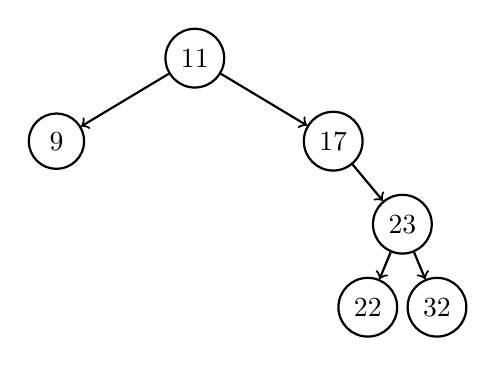
\begin{tikzpicture}[
        invis/.style={draw=none},
        every node/.style={draw, circle, minimum size=20pt, text centered, thick},
        edge from parent/.style ={draw, ->, thick},
        level 1/.style={sibling distance=100pt},
        level 2/.style={sibling distance=50pt},
        level 3/.style={sibling distance=25pt},
        level distance=30pt,
    ]
    \node[](root){11}
    child{node[](9){9}}
    child{node[](17){17}
        child{node[invis]{} edge from parent [draw=none]}
        child{node[](23){23}
            child{node[](22){22}}
            child{node[](32){32}}
        }
    }
    ;

    \end{tikzpicture}
    \captionof*{figure}{Splay 11 (zigzag)}
\end{minipage}

\textbf{Insert:}

\begin{minipage}[t]{0.5\textwidth}
    \centering
    \begin{tikzpicture}[
        invis/.style={draw=none},
        every node/.style={draw, circle, minimum size=20pt, text centered, thick},
        edge from parent/.style ={draw, ->, thick},
        level 1/.style={sibling distance=100pt},
        level 2/.style={sibling distance=50pt},
        level 3/.style={sibling distance=25pt},
        level distance=30pt,
    ]
    \node[](root){17}
    child{node[](9){9}
        child{node[](6){6}}
        child{node[](11){11}}
    }
    child{node[](23){23}
        child{node[](22){22}}
        child{node[](32){32}}
    }
    ;
    \draw[->, codegreen, very thick] (root) to (9);
    \draw[->, codegreen, very thick] (9) to (6);

    \end{tikzpicture}
    \captionof*{figure}{Insert 6}
\end{minipage}
\begin{minipage}[t]{0.5\textwidth}
    \centering
    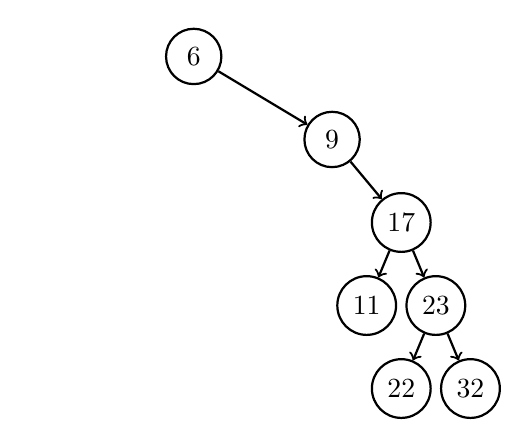
\begin{tikzpicture}[
        invis/.style={draw=none},
        every node/.style={draw, circle, minimum size=20pt, text centered, thick},
        edge from parent/.style ={draw, ->, thick},
        level 1/.style={sibling distance=100pt},
        level 2/.style={sibling distance=50pt},
        level 3/.style={sibling distance=25pt},
        level distance=30pt,
    ]
    \node[](root){6}
    child{node[invis]{} edge from parent [draw=none]}
    child{node[](9){9}
        child{node[invis]{} edge from parent [draw=none]}
        child{node[](17){17}
            child{node[](11){11}}
            child{node[](23){23}
                child{node[](22){22}}
                child{node[](32){32}}
            }
        }
    }
    ;

    \end{tikzpicture}
    \captionof*{figure}{Splay 6 (zigzig)}
\end{minipage}

\textbf{Delete:}

\begin{minipage}[t]{\textwidth}
    \centering
    \begin{tikzpicture}[
        invis/.style={draw=none},
        every node/.style={draw, circle, minimum size=20pt, text centered, thick},
        edge from parent/.style ={draw, ->, thick},
        level 1/.style={sibling distance=100pt},
        level 2/.style={sibling distance=50pt},
        level 3/.style={sibling distance=25pt},
        level distance=30pt,
    ]
    \node[](root){17}
    child{node[](9){9}
        child{node[](6){6}}
        child{node[](11){11}}
    }
    child{node[](23){23}
        child{node[](22){22}}
        child{node[](32){32}}
    }
    ;
    \draw[->, codegreen, thick, bend right] (root) to (9);
    \draw[->, codegreen, thick, bend right] (23) to (root);
    \draw[->, codegreen, very thick] (22) to (11);
    \end{tikzpicture}
    \captionof*{figure}{Before delete 23}
\end{minipage}
\begin{minipage}[t]{0.5\textwidth}
    \centering
    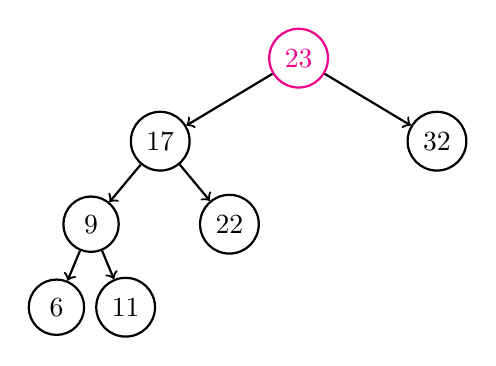
\begin{tikzpicture}[
        invis/.style={draw=none},
        every node/.style={draw, circle, minimum size=20pt, text centered, thick},
        edge from parent/.style ={draw, ->, thick},
        level 1/.style={sibling distance=100pt},
        level 2/.style={sibling distance=50pt},
        level 3/.style={sibling distance=25pt},
        level distance=30pt,
    ]
    \node[magenta](root){23}
    child{node[](17){17}
        child{node[](9){9}
            child{node[](6){6}}
            child{node[](11){11}}
        }
        child{node[](22){22}}
    }
    child{node[](32){32}}
    ;
    
    \end{tikzpicture}
    \captionof*{figure}{Splay 23 (zig)}
\end{minipage}
\begin{minipage}[t]{0.5\textwidth}
    \centering
    \begin{tikzpicture}[
        invis/.style={draw=none},
        every node/.style={draw, circle, minimum size=20pt, text centered, thick},
        edge from parent/.style ={draw, ->, thick},
        level 1/.style={sibling distance=100pt},
        level 2/.style={sibling distance=50pt},
        level 3/.style={sibling distance=25pt},
        level distance=30pt,
    ]
    \node[invis](root){}
    child{node[](17){17} edge from parent [draw=none]
        child{node[](9){9}
            child{node[](6){6}}
            child{node[](11){11}}
        }
        child{node[](22){22}}
    }
    child{node[](32){32} edge from parent [draw=none]}
    ;
    \draw[->, codegreen, thick, bend right] (22) to (17);
    \draw[->, codegreen, thick, bend right] (17) to (9);
    \draw[->, codegreen, thick, bend right, out=290] (22) to (32);
    \end{tikzpicture}
    \captionof*{figure}{delete 23}
\end{minipage}
\begin{minipage}[t]{\textwidth}
    \centering
    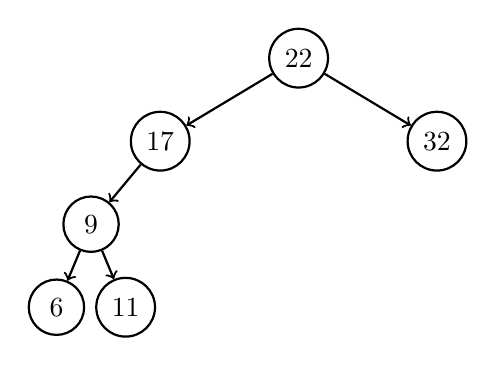
\begin{tikzpicture}[
        invis/.style={draw=none},
        every node/.style={draw, circle, minimum size=20pt, text centered, thick},
        edge from parent/.style ={draw, ->, thick},
        level 1/.style={sibling distance=100pt},
        level 2/.style={sibling distance=50pt},
        level 3/.style={sibling distance=25pt},
        level distance=30pt,
    ]
    \node[](root){22}
    child{node[](17){17}
        child{node[](9){9}
            child{node[](6){6}}
            child{node[](11){11}}
        }
        child{node[invis]{} edge from parent [draw=none]}
    }
    child{node[](32){32}}
    ;

    \end{tikzpicture}
    \captionof*{figure}{Splay biggest node in left subtree (22) and append right subtree}
\end{minipage}

Eine schöne interaktive Visualisierung von Splay Trees kann man \href{https://www.cs.usfca.edu/~galles/visualization/SplayTree.html}{hier} finden.

\includepdf[pages={73,77}, pagecommand={},nup=1x2, frame=true, scale=0.9]{../VL_Folien/04AdvancedDataStructures.pdf}
\subsection{Binary Heap Trees}
Im Allgemeinen ist ein Binary Heap wie folgt definiert:
\begin{itemize}
    \item Bis auf das unterste Level ist der Baum vollständig gefüllt und im untersten Level ist er von links befüllt.
    \item $\forall x \neq root: x.parent.key \geq x.key$
\end{itemize}
Binary Heaps unterscheiden sich von den anderen hier behandelten Trees insofern, dass sie keine BSTs sind. Das heißt, dass rechte Kinder eines Knotens nicht unbedingt größer als dieser sind und linke Kinder dieses Knotens nicht unbedingt kleiner. Sie sind so organiesiert, dass sie Werte nach Ebenen sortieren. Bei Max heaps zum Beispiel steht der größte Wert in der Wurzel und der kleinste Wert irgendwo in der untersten Ebene. So ergibt sich bei Max heaps also die Eigenschaft, dass die parent node einer node immer größer ist als die node selber. Dies erlaubt einen sehr schnellen Zugriff auf das größte Element. Diese Eigenschaft kann sehr gut genutzt werden um Werte zu sortieren. Zudem sind Binary Heaps anders konstruiert als andere Trees, sie besitzen nämlich keine Nodes perse, sondern sind nur über Positionen in einem array gespeichert. Die Beziehungen zwischen den Nodes ergeben sich durch Formeln:
\begin{itemize}
    \item \textbf{Parent}: $parent(i) = \lceil i / 2 \rceil -1$
    \item \textbf{Left Child}: $left(i) = (2 \cdot i) + 1$
    \item \textbf{Right Child}: $right(i) = 2 \cdot (i + 1)$
\end{itemize}

\textbf{Definition and standard Operations:}

\begin{algorithm}[H]
    \SetKwFunction{KwBinaryMaxHeap}{BinaryMaxHeap}
    \SetKwFunction{KwarrayToHeap}{arrayToHeap}
    \SetKwFunction{Kwparent}{parent}
    \SetKwFunction{Kwleft}{left}
    \SetKwFunction{Kwright}{right}
    \SetKwFunction{KwisEmpty}{isEmpty}
    \Cl{\KwBinaryMaxHeap{}}{
        heap\;
        size\;
        \Con{\KwBinaryMaxHeap{n}}{
            heap = \text{new array of size } $n$\;
            size = $0$\;
        }
        \Con{\KwBinaryMaxHeap{arr}}{
            \KwarrayToHeap{arr}\;
        }
        \Fn{\KwarrayToHeap{arr}}{
            heap = arr.clone()\;
            size = $0$\;
            \ForEach{i $\in$ arr}{
                \If{i $==$ \KwNil}{
                    \KwBreak\;
                }
                size = $size + 1$\;
            }
        }
        \tcp{Complexity: O(1)}
        \Fn{\Kwparent{i}}{
            \KwRet $\lceil i/2 \rceil - 1$\;
        }
        \tcp{Complexity: O(1)}
        \Fn{\Kwleft{i}}{
            \KwRet $(2 \cdot i) + 1$\;
        }
        \tcp{Complexity: O(1)}
        \Fn{\Kwright{i}}{
            \KwRet $2 \cdot (i + 1)$\;
        }
        \tcp{Complexity: O(1)}
        \Fn{\KwisEmpty{}}{
            \KwRet $size == 0$\;
        }
    }
\end{algorithm}

\begin{minipage}[t]{\textwidth}
    \centering
    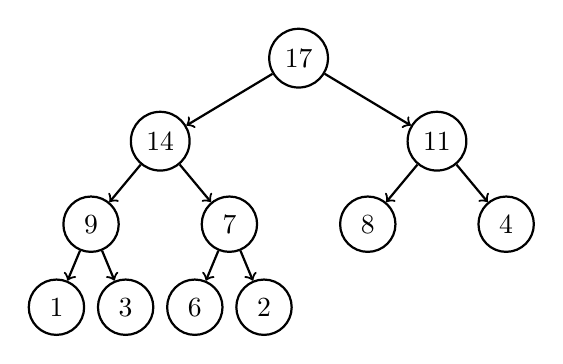
\begin{tikzpicture}[
        invis/.style={draw=none},
        every node/.style={draw, circle, minimum size=20pt, text centered, thick},
        edge from parent/.style ={draw, ->, thick},
        level 1/.style={sibling distance=100pt},
        level 2/.style={sibling distance=50pt},
        level 3/.style={sibling distance=25pt},
        level distance=30pt,
    ]
    \node[](root){17}
    child{node[](14){14}
        child{node[](9){9}
            child{node[](1){1}}
            child{node[](3){3}}
        }
        child{node[](7){7}
            child{node[](6){6}}
            child{node[](2){2}}
        }
    }
    child{node[](11){11}
        child{node[](8){8}}
        child{node[](4){4}}
    }
    ;
    \end{tikzpicture}
\end{minipage}\\
\begin{minipage}[t]{\textwidth}
    \centering
    \begin{tikzpicture}[
        array/.style={
            matrix of nodes, nodes={draw ,minimum width = 30pt, minimum height = 15pt, fill=backcolour, anchor=center},
            row 1/.style={nodes={draw=none, fill=none, color=codegray}},
        },
    ]
    \matrix[array](heap){
        0  & 1  & 2  & 3  & 4  & 5  & 6  & 7  & 8  & 9  & 10 & ...\\
        17 & 14 & 11 & 9  & 7  & 8  & 4  & 1  & 3  & 6  & 2  & nil\\
    };
    \end{tikzpicture}
\end{minipage}

\textbf{Insert:}

\begin{algorithm}[H]
    \SetKwFunction{KwBinaryMaxHeap}{BinaryMaxHeap}
    \SetKwFunction{Kwinsert}{insert}
    \SetKwFunction{Kwparent}{parent}
    \Cl{\KwBinaryMaxHeap{} \textnormal{(continued)}}{
        \tcp{Complexity: O(h) = O(log n)}
        \Fn{\Kwinsert{k}}{
            size = $size + 1$\;
            heap[$size - 1$] = k; \tcp{Add new element at first empty index}
            i = $size - 1$\;
            \While{$i > 0$ \KwAnd heap[$i$] $>$ heap[\Kwparent{i}]}{
                \tcp{Moves upward through tree}
                Swap heap[$i$] with heap[\Kwparent{i}]\;
                i = \Kwparent{i}; \tcp{Move up}
            }
        }
    }
\end{algorithm}

Für min Heaps muss lediglich das Ungleichheitszeichen umgedreht werden. \\
\begin{minipage}[t]{0.5\textwidth}
    \centering
    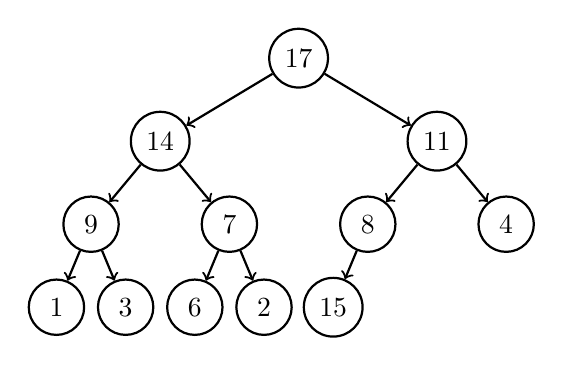
\begin{tikzpicture}[
        invis/.style={draw=none},
        every node/.style={draw, circle, minimum size=20pt, text centered, thick},
        edge from parent/.style ={draw, ->, thick},
        level 1/.style={sibling distance=100pt},
        level 2/.style={sibling distance=50pt},
        level 3/.style={sibling distance=25pt},
        level distance=30pt,
    ]
    \node[](root){17}
    child{node[](14){14}
        child{node[](9){9}
            child{node[](1){1}}
            child{node[](3){3}}
        }
        child{node[](7){7}
            child{node[](6){6}}
            child{node[](2){2}}
        }
    }
    child{node[](11){11}
        child{node[](8){8}
            child{node[](15){15}}
            child{node[invis]{} edge from parent [draw=none]}
        }
        child{node[](4){4}}
    }
    ;
    \end{tikzpicture}
    \captionof*{figure}{Insert 15, before fixup}
\end{minipage}
\begin{minipage}[t]{0.5\textwidth}
    \centering
    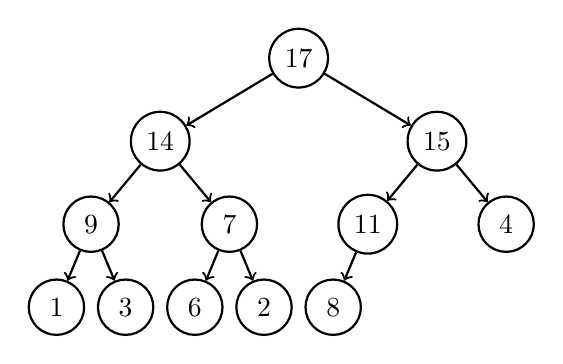
\begin{tikzpicture}[
        invis/.style={draw=none},
        every node/.style={draw, circle, minimum size=20pt, text centered, thick},
        edge from parent/.style ={draw, ->, thick},
        level 1/.style={sibling distance=100pt},
        level 2/.style={sibling distance=50pt},
        level 3/.style={sibling distance=25pt},
        level distance=30pt,
    ]
    \node[](root){17}
    child{node[](14){14}
        child{node[](9){9}
            child{node[](1){1}}
            child{node[](3){3}}
        }
        child{node[](7){7}
            child{node[](6){6}}
            child{node[](2){2}}
        }
    }
    child{node[](15){15}
        child{node[](11){11}
            child{node[](8){8}}
            child{node[invis]{} edge from parent [draw=none]}
        }
        child{node[](4){4}}
    }
    ;
    \end{tikzpicture}
    \captionof*{figure}{After fixup}
\end{minipage}

\newpage
\textbf{Heapify:}

\begin{algorithm}[H]
    \SetKwFunction{KwBinaryMaxHeap}{BinaryMaxHeap}
    \SetKwFunction{Kwheapify}{heapify}
    \SetKwFunction{Kwleft}{left}
    \SetKwFunction{Kwright}{right}
    \Cl{\KwBinaryMaxHeap{} \textnormal{(continued)}}{
        \tcp{Complexity: O(h) = O(log n)}
        \Fn{\Kwheapify{i}}{
            max = i\;
            l = \Kwleft{i}\;
            r = \Kwright{i}\;
            \If{$l < size$ \KwAnd heap[$i$] $<$ heap[$l$]}{
                max = l; \tcp{Set max to left}
            }
            \If{$r < size$ \KwAnd heap[$max$] $<$ heap[$r$]}{
                max = r; \tcp{if right child is bigger than max (i or left)}
            }
            \If{$max \neq i$}{
                \tcp{If max is not i -> max is left or right}
                Swap heap[$i$] with heap[$max$]\;
                \Kwheapify{max}; \tcp{Move down the tree}
            }
        }
    }
\end{algorithm}

Tut essenziell das selbe wie der zweite Teil von Insert, nur in umgekehrter Reihenfolge (oben nach unten) und rekursiv.\\ 
Für Min heap muss wieder das Gleichheitszeichen umgedreht werden.\\
\begin{minipage}[t]{0.5\textwidth}
    \centering
    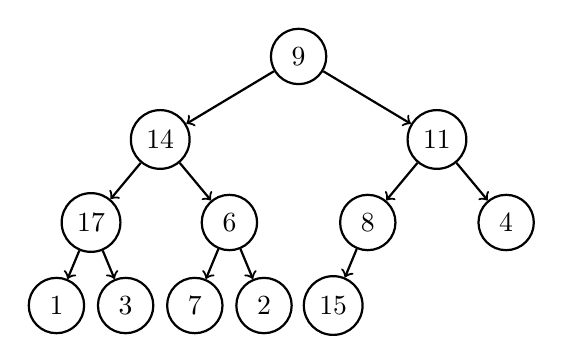
\begin{tikzpicture}[
        invis/.style={draw=none},
        every node/.style={draw, circle, minimum size=20pt, text centered, thick},
        edge from parent/.style ={draw, ->, thick},
        level 1/.style={sibling distance=100pt},
        level 2/.style={sibling distance=50pt},
        level 3/.style={sibling distance=25pt},
        level distance=30pt,
    ]
    \node[](root){9}
    child{node[](14){14}
        child{node[](17){17}
            child{node[](1){1}}
            child{node[](3){3}}
        }
        child{node[](6){6}
            child{node[](7){7}}
            child{node[](2){2}}
        }
    }
    child{node[](11){11}
        child{node[](8){8}
            child{node[](15){15}}
            child{node[invis]{} edge from parent [draw=none]}
        }
        child{node[](4){4}}
    }
    ;
    \end{tikzpicture}
    \captionof*{figure}{Before}
\end{minipage}
\begin{minipage}[t]{0.5\textwidth}
    \centering
    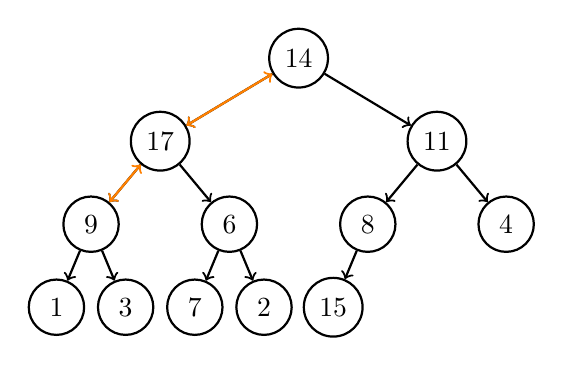
\begin{tikzpicture}[
        invis/.style={draw=none},
        every node/.style={draw, circle, minimum size=20pt, text centered, thick},
        edge from parent/.style ={draw, ->, thick},
        level 1/.style={sibling distance=100pt},
        level 2/.style={sibling distance=50pt},
        level 3/.style={sibling distance=25pt},
        level distance=30pt,
    ]
    \node[](root){14}
    child{node[](17){17}
        child{node[](9){9}
            child{node[](1){1}}
            child{node[](3){3}}
        }
        child{node[](6){6}
            child{node[](7){7}}
            child{node[](2){2}}
        }
    }
    child{node[](11){11}
        child{node[](8){8}
            child{node[](15){15}}
            child{node[invis]{} edge from parent [draw=none]}
        }
        child{node[](4){4}}
    }
    ;
    \draw[<->, orange, thick] (root) to (17);
    \draw[<->, orange, thick] (17) to (9);
    \end{tikzpicture}
    \captionof*{figure}{Heapify root}
\end{minipage}

\newpage
\textbf{Build Heap and Heap Sort:}

\begin{algorithm}[H]
    \SetKwFunction{KwBinaryMaxHeap}{BinaryMaxHeap}
    \SetKwFunction{KwbuildHeap}{buildHeap}
    \SetKwFunction{KwheapSort}{heapSort}
    \SetKwFunction{KwextractMax}{extractMax}
    \SetKwFunction{Kwparent}{parent}
    \SetKwFunction{Kwheapify}{heapify}
    \SetKwFunction{KwisEmpty}{isEmpty}
    \Cl{\KwBinaryMaxHeap{} \textnormal{(continued)}}{
        \tcp{Complexity: O(n)}
        \Fn{\KwbuildHeap{}}{
            \For{i = \Kwparent{$size - 1$} \KwDownTo $0$}{
                \Kwheapify{i}; \tcp{Calls heapify on each node starting from second to last row}
            }
        }
        \tcp{Complexity: O(n log n)}
        \Fn{\KwheapSort{}}{
            \KwbuildHeap{}; \tcp{Sorts heap accordingly}
            res = \text{new array of size } $size$; \tcp{Create new array for sorted result}
            i = $0$\;
            \While{\KwNot \KwisEmpty{}}{
                res[$i$] = \KwextractMax{}; \tcp{Extract max and add to array}
                i = $i + 1$\;
            }
            \KwRet res; \tcp{Array is now sorted in reverse natural order}
        }
        \tcp{Complexity: O(h) = O(log n)}
        \Fn{\KwextractMax{}}{
            \If{\KwisEmpty{}}{
                \KwRet \KwError; \tcp{Underflow check}
            }
            max = heap[$0$]; \tcp{Biggest value at root}
            heap[$0$] = heap[$size - 1$]; \tcp{Sets root to last element}
            size = $size - 1$; \tcp{Decrease size}
            \Kwheapify{$0$}; \tcp{Heapify new root}
            \KwRet max\;
        }
    }
\end{algorithm}

\begin{minipage}[t]{0.5\textwidth}
    \centering
    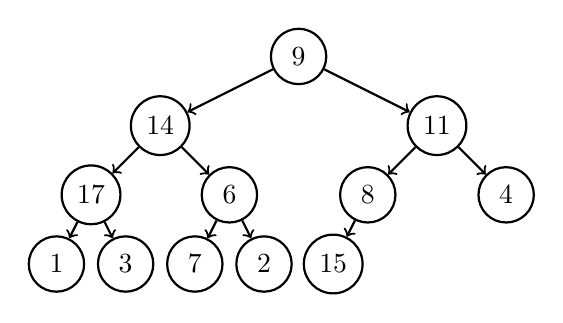
\begin{tikzpicture}[
        invis/.style={draw=none},
        every node/.style={draw, circle, minimum size=20pt, text centered, thick},
        edge from parent/.style ={draw, ->, thick},
        level 1/.style={sibling distance=100pt},
        level 2/.style={sibling distance=50pt},
        level 3/.style={sibling distance=25pt},
        level distance=25pt,
    ]
    \node[](root){9}
    child{node[](14){14}
        child{node[](17){17}
            child{node[](1){1}}
            child{node[](3){3}}
        }
        child{node[](6){6}
            child{node[](7){7}}
            child{node[](2){2}}
        }
    }
    child{node[](11){11}
        child{node[](8){8}
            child{node[](15){15}}
            child{node[invis]{} edge from parent [draw=none]}
        }
        child{node[](4){4}}
    }
    ;
    \end{tikzpicture}
    \captionof*{figure}{Before heapsort}
\end{minipage}
\begin{minipage}[t]{0.5\textwidth}
    \centering
    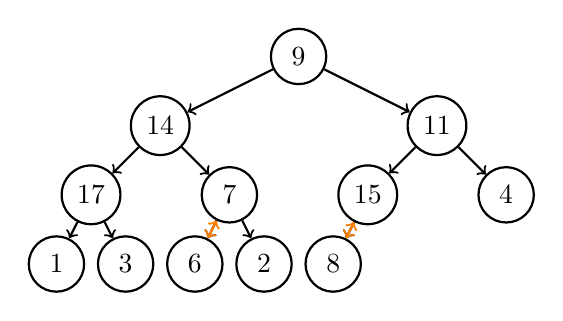
\begin{tikzpicture}[
        invis/.style={draw=none},
        every node/.style={draw, circle, minimum size=20pt, text centered, thick},
        edge from parent/.style ={draw, ->, thick},
        level 1/.style={sibling distance=100pt},
        level 2/.style={sibling distance=50pt},
        level 3/.style={sibling distance=25pt},
        level distance=25pt,
    ]
    \node[](root){9}
    child{node[](14){14}
        child{node[](17){17}
            child{node[](1){1}}
            child{node[](3){3}}
        }
        child{node[](7){7}
            child{node[](6){6}}
            child{node[](2){2}}
        }
    }
    child{node[](11){11}
        child{node[](15){15}
            child{node[](8){8}}
            child{node[invis]{} edge from parent [draw=none]}
        }
        child{node[](4){4}}
    }
    ;
    \draw[<->, orange, thick] (6) to (7);
    \draw[<->, orange, thick] (15) to (8);
    \end{tikzpicture}
    \captionof*{figure}{heapify second to last level}
\end{minipage}
\begin{minipage}[t]{0.5\textwidth}
    \centering
    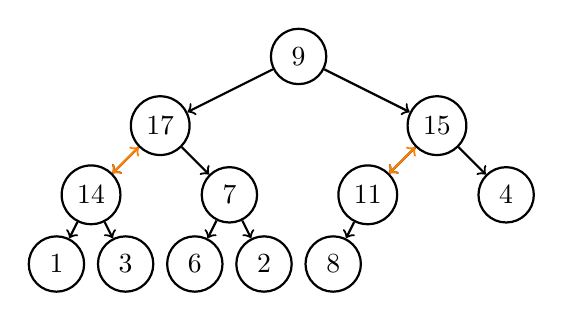
\begin{tikzpicture}[
        invis/.style={draw=none},
        every node/.style={draw, circle, minimum size=20pt, text centered, thick},
        edge from parent/.style ={draw, ->, thick},
        level 1/.style={sibling distance=100pt},
        level 2/.style={sibling distance=50pt},
        level 3/.style={sibling distance=25pt},
        level distance=25pt,
    ]
    \node[](root){9}
    child{node[](17){17}
        child{node[](14){14}
            child{node[](1){1}}
            child{node[](3){3}}
        }
        child{node[](7){7}
            child{node[](6){6}}
            child{node[](2){2}}
        }
    }
    child{node[](15){15}
        child{node[](11){11}
            child{node[](8){8}}
            child{node[invis]{} edge from parent [draw=none]}
        }
        child{node[](4){4}}
    }
    ;
    \draw[<->, orange, thick] (17) to (14);
    \draw[<->, orange, thick] (15) to (11);
    \end{tikzpicture}
    \captionof*{figure}{heapify third to last level}
\end{minipage}
\begin{minipage}[t]{0.5\textwidth}
    \centering
    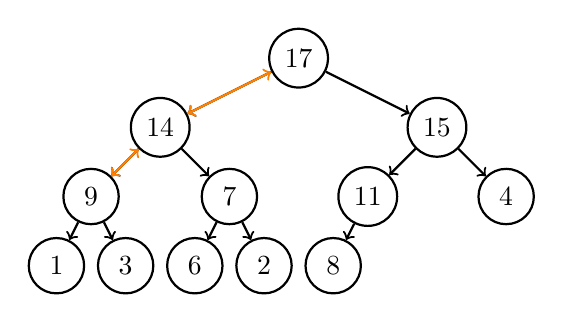
\begin{tikzpicture}[
        invis/.style={draw=none},
        every node/.style={draw, circle, minimum size=20pt, text centered, thick},
        edge from parent/.style ={draw, ->, thick},
        level 1/.style={sibling distance=100pt},
        level 2/.style={sibling distance=50pt},
        level 3/.style={sibling distance=25pt},
        level distance=25pt,
    ]
    \node[](root){17}
    child{node[](14){14}
        child{node[](9){9}
            child{node[](1){1}}
            child{node[](3){3}}
        }
        child{node[](7){7}
            child{node[](6){6}}
            child{node[](2){2}}
        }
    }
    child{node[](15){15}
        child{node[](11){11}
            child{node[](8){8}}
            child{node[invis]{} edge from parent [draw=none]}
        }
        child{node[](4){4}}
    }
    ;
    \draw[<->, orange, thick] (root) to (14);
    \draw[<->, orange, thick] (14) to (9);
    \end{tikzpicture}
    \captionof*{figure}{heapify last level}
\end{minipage}\\
\begin{minipage}[t]{\textwidth}
    \centering
    \begin{tikzpicture}[
        array/.style={
            matrix of nodes, nodes={draw ,minimum width = 30pt, minimum height = 15pt, fill=backcolour, anchor=center},
            row 1/.style={nodes={draw=none, fill=none, color=codegray}},
        },
    ]
    \matrix[array](heap){
        0  & 1  & 2  & 3  & 4  & 5  & 6  & 7  & 8  & 9  & 10 & 11\\
        17 & 15 & 14 & 11 & 9  & 8  & 7  & 6  & 4  & 3  & 2  & 1 \\
    };
    \end{tikzpicture}
    \captionof*{figure}{Extracted array}
\end{minipage}

Eine schöne interaktive Visualisierung von Splay Trees kann man \href{https://www.crackr.dev/visualize/max-heap}{hier} finden.
\includepdf[pages={92,94,96,101}, pagecommand={},nup=2x2, frame=true, scale=0.9]{../VL_Folien/04AdvancedDataStructures.pdf}
\subsection{B-Tree}
B-Trees (B hat keine festgelegte Bedeutung) unterscheiden sich sehr von den anderen Trees. Erstens sind sie keine Binary Trees. Ein B-Tree vom Grad $t$ wird so definiert, dass
\begin{itemize}
    \item Jede Node besitzt minimal $t - 1$ Werte und $t$ Kinder (Außer root)
    \item Jede Node besitzt maximal $2\cdot t - 1$ Werte und $2\cdot t$ Kinder
    \item Die Werte innerhalb eines Knotens sind aufsteigend sortiert
    \item Alle Blätter haben die gleiche Höhe
    \item Jeder innere Knoten mit m Werten hat m + 1 Kinder \\ $\implies$ für alle Werte $k_j$ in j-ten Kind gilt: $k_0 \leq key[0] \leq k_1 \leq key[1] \leq \ldots \leq key[m-1] \leq k_m $
\end{itemize}
Ein B-Tree kann somit in einem Knoten mehr als einen Wert und mehr als zwei Kinder besitzen. B-Trees balanzieren sich zudem auch selber, wodurch sie sehr effektiv Operationen in logarithmischer Laufzeit ausführen. Zudem ist durch die Anzahl der Werte die in einem Knoten gespeichert werden können und die Anzahl an Kinder die ein Knoten haben kann die Höhe des Baumes deutlich niedriger. B-Trees bieten sich so sehr für Disk-Based Operationen an, da sie die Anzahl an Disk-Access reduziert im Vergleich zu anderen Trees. Sie bieten sich also besonders für sehr große Datenbanken auf Festplatten an, sind aber im Vergleich zu den anderen Trees bei kleineren Eingaben weniger effizient.
Die maximale Höhe von B Trees ist $ h = \leq \log_t(\frac{n + 1}{2})$.
\begin{minipage}[t]{\textwidth}
    \centering
    \begin{tikzpicture}[
        array/.style={
            matrix, matrix of nodes, ampersand replacement=\&, grow= right, nodes={draw, minimum width = 20pt, minimum height = 15pt, fill=backcolour, anchor=center,},
        },
        edge from parent/.style ={draw, ->, very thick},
        level 1/.style={sibling distance=170pt},
        level 2/.style={sibling distance=60pt},
        level 3/.style={sibling distance=30pt},
        level distance=40pt,
    ]
    \node[array](root){34\\}
    child{node[array](){
            5 \& 13\\
        }
        child{node[array](){
            1 \& 2 \& 4\\
            }
        }
        child{node[array](){
            6 \& 7\\
            }
        }
        child{node[array](){
            17 \& 21 \& 23\\
            }
        }
    }
    child{node[array](){
            53\\
        }
        child{node[array](){
            37 \& 42 \& 44\\
            }
        }
        child{node[array](){
            59 \& 67\\
            }
        }
    }
    ;
    \end{tikzpicture}
    \captionof*{figure}{B-Tree example (Degree $t = 2$)}
\end{minipage}

\textbf{Definition and Search:}

\begin{algorithm}[H]
    \SetKwFunction{KwBTree}{BTree}
    \SetKwFunction{KwBNode}{BNode}
    \SetKwFunction{KwfindKey}{findKey}
    \SetKwFunction{KwinNode}{inNode}
    \SetKwFunction{Kwtraverse}{traverse}
    \SetKwFunction{Kwsearch}{search}
    \Cl{\KwBTree{}}{
        root\;
        t\;
        \Con{\KwBTree{t}}{
            root = \KwNil\;
            this.t = t\;
        }
        \Fn{\Kwsearch{k}}{
            \If{root $==$ \KwNil}{
                \KwPrint \text{"Tree is empty"}\;
                \KwRet\;
            }
            root.\Kwsearch{k}\;
        }
        \Fn{\Kwtraverse{}}{
            \If{root $\neq$ \KwNil}{
                root.\Kwtraverse{}\;
            }
        }
    }
\end{algorithm}

\begin{algorithm}[H]
    \setcounter{AlgoLine}{14}
    \SetKwFunction{KwBTree}{BTree}
    \SetKwFunction{KwBNode}{BNode}
    \SetKwFunction{KwfindKey}{findKey}
    \SetKwFunction{KwinNode}{inNode}
    \SetKwFunction{Kwtraverse}{traverse}
    \SetKwFunction{Kwsearch}{search}
    \Cl{\KwBNode{}}{
        keys\;
        t\;
        children\;
        n\;
        isLeaf\;
        \Con{\KwBNode{t, isLeaf}}{
            keys = \text{new array of size } $2 \cdot t - 1$\;
            this.t = t\;
            children = \text{new array of size } $2 \cdot t$; \tcp{1 more than keys}
            n = $0$\;
            this.isLeaf = isLeaf\;
        }
        \Fn{\KwfindKey{k}}{
            i = $0$\;
            \While{$i < n$ \KwAnd $keys[i] < k$}{
                i = $i + 1$\;
            }
            \KwRet i\;
        }
        \Fn{\KwinNode{i, k}}{
            \KwRet $i < n$ \KwAnd $keys[i] == k$\;
        }
        \Fn{\Kwtraverse{}}{
            \For{$i = 0$ \KwTo $n - 1$}{
                \If{\KwNot isLeaf}{
                    children[$i$].\Kwtraverse{}\;
                }
                \KwPrint keys[$i$]\;
            }
            \If{\KwNot isLeaf}{
                children[$n$].\Kwtraverse{}\;
            }
        }
        \Fn{\Kwsearch{k}}{
            i = \KwfindKey{k}\;
            \If{\KwinNode{i, k}}{
                \KwRet this\;
            }
            \If{isLeaf}{
                \KwRet \KwNil\;
            }
            \KwRet children[$i$].\Kwsearch{k}\;
        }
    }
\end{algorithm}


Der Suchalgorithmus ist relativ simpel. Er durchläuft die key-Werte der Wurzel, bis es beim Element angelangt, das größer oder gleich dem Suchwert ist. Ist der Wert gleich, so gibt es den Knoten zurück. Andernfalls, wenn der Knoten keine Kinder hat, existiert der Wert nicht, ansonsten durchsucht der Algorithmus das Kind, das den Wert beinhalten sollte rekursiv.


\begin{minipage}[t]{\textwidth}
    \centering
    \begin{tikzpicture}[
        array/.style={
            matrix, matrix of nodes, ampersand replacement=\&, grow= right, nodes={draw, minimum width = 20pt, minimum height = 15pt, fill=backcolour, anchor=center,},
        },
        edge from parent/.style ={draw, ->, very thick},
        level 1/.style={sibling distance=170pt},
        level 2/.style={sibling distance=60pt},
        level 3/.style={sibling distance=30pt},
        level distance=40pt,
    ]
    \node[array](root){34\\}
    child{node[array](l){
            5 \& 13\\
        }
        child{node[array](ll){
            1 \& 2 \& 4\\
            }
        }
        child{node[array](lm){
            6 \& 7\\
            }
        }
        child{node[array](lr){
            17 \& 21 \& 23\\
            }
        }
    }
    child{node[array](r){
            53\\
        }
        child{node[array](rl){
            37 \& 42 \& 44\\
            }
        }
        child{node[array](rr){
            59 \& 67\\
            }
        }
    }
    ;
    \draw[->, codegreen, thick, bend right] (root) to (l-1-1.north);
    \draw[->, codegreen, thick, bend left=45] (l-1-1.north) to (l-1-2.north);
    \draw[->, codegreen, thick, bend left] (l-1-2.east) to (lr-1-1.north);
    \draw[->, codegreen, thick, bend left=45] (lr-1-1.north) to (lr-1-2.north);

    \end{tikzpicture}
    \captionof*{figure}{Search 21}
\end{minipage}

\newpage
\textbf{Insertion:}

\begin{algorithm}[H]
    \SetKwFunction{KwBTree}{BTree}
    \SetKwFunction{KwBNode}{BNode}
    \SetKwFunction{Kwinsert}{insert}
    \SetKwFunction{KwinsertNonFull}{insertNonFull}
    \SetKwFunction{KwsplitChild}{splitChild}
    \Cl{\KwBNode{} \textnormal{(continued)}}{
        \tcp{Complexity: O(t)}
        \Fn{\KwinsertNonFull{k}}{
            i = $n - 1$\;
            \If{isLeaf}{
                \While{$i \geq 0$ \KwAnd $keys[i] > k$}{
                    keys[$i + 1$] = keys[$i$]\;
                    i = $i - 1$\;
                }
                keys[$i + 1$] = k\;
                n = $n + 1$\;
            }
            \Else{
                \While{$i \geq 0$ \KwAnd $keys[i] > k$}{
                    i = $i - 1$\;
                }
                \If{children[$i + 1$].n $== 2 \cdot t - 1$}{
                    \KwsplitChild{$i + 1$, children[$i + 1$]}\;
                    \If{$keys[i + 1] < k$}{
                        i = $i + 1$\;
                    }
                }
                children[$i + 1$].\KwinsertNonFull{k}\;
            }
        }
        \Fn{\KwsplitChild{i, y}}{
            z = \text{new } BNode(y.t, y.isLeaf)\;
            z.n = $t - 1$\;
            \For{$j = 0$ \KwTo $t - 2$}{
                z.keys[$j$] = y.keys[$j + t$]\;
            }
            \If{\KwNot y.isLeaf}{
                \For{$j = 0$ \KwTo $t - 1$}{
                    z.children[$j$] = y.children[$j + t$]\;
                }
            }
            y.n = $t - 1$\;
            \For{$j = n$ \KwDownTo $i + 1$}{
                children[$j + 1$] = children[$j$]\;
            }
            children[$i + 1$] = z\;
            \For{$j = n - 1$ \KwDownTo i}{
                keys[$j + 1$] = keys[$j$]\;
            }
            keys[$i$] = y.keys[$t - 1$]\;
            n = $n + 1$\;
        }
    }
\end{algorithm}

\begin{algorithm}[H]
    \setcounter{AlgoLine}{34}
    \SetKwFunction{KwBTree}{BTree}
    \SetKwFunction{KwBNode}{BNode}
    \SetKwFunction{Kwinsert}{insert}
    \SetKwFunction{KwinsertNonFull}{insertNonFull}
    \SetKwFunction{KwsplitChild}{splitChild}
    \Cl{\KwBTree{} \textnormal{(continued)}}{
        \Fn{\Kwinsert{k}}{
            \If{root $==$ \KwNil}{
                root = \text{new } BNode(t, \KwTrue)\;
                root.keys[$0$] = k\;
                root.n = $1$\;
            }
            \Else{
                \If{root.n $== 2 \cdot t - 1$}{
                    s = \text{new } BNode(t, \KwFalse)\;
                    s.children[$0$] = root\;
                    s.\KwsplitChild{$0$, root}\;
                    i = $0$\;
                    \If{s.keys[$0$] $<$ k}{
                        i = $i + 1$\;
                    }
                    s.children[$i$].\KwinsertNonFull{k}\;
                    root = s\;
                }
                \Else{
                    root.\KwinsertNonFull{k}\;
                }
            }
        }
    }
\end{algorithm}


Prinzipiell folgt dieser Algorithmus einfach der Folge: 
\begin{enumerate}
    \item Finde Einfügepunkt
    \item Wenn Node schon $2 \cdot t -1 $ Werte besitzt, splitte es
    \begin{itemize}
        \item Teile Node in zwei Nodes mit je $ t - 1 $ Werten
        \item Der mittlere Knoten wird in den Elternknoten eingefügt
        \item Wenn dadurch der Elternknoten $2 \cdot t - 1 $ Werte besitzt, splitte diesen rekursiv nach oben 
    \end{itemize}
    \item Wert am Einfügepunkt einfügen
\end{enumerate}

\begin{minipage}[t]{\textwidth}
    \centering
    \begin{tikzpicture}[
        array/.style={
            matrix, matrix of nodes, ampersand replacement=\&, grow= right, nodes={draw, minimum width = 20pt, minimum height = 15pt, fill=backcolour, anchor=center,},
        },
        edge from parent/.style ={draw, ->, very thick},
        level 1/.style={sibling distance=170pt},
        level 2/.style={sibling distance=70pt},
        level 3/.style={sibling distance=30pt},
        level distance=40pt,
    ]
    \node[array](root){34\\}
    child{node[array](l){
            5 \& 13\\
        }
        child{node[array](ll){
            1 \& 2 \& 4\\
            }
        }
        child{node[array](lm){
            6 \& 7 \& 9\\
            }
        }
        child{node[array](lr){
            17 \& 21 \& 23\\
            }
        }
    }
    child{node[array](r){
            53\\
        }
        child{node[array](rl){
            37 \& 42 \& 44\\
            }
        }
        child{node[array](rr){
            59 \& 67\\
            }
        }
    }
    ;
    \draw[->, codegreen, thick, bend right] (root) to (l-1-2.north);
    \draw[->, codegreen, thick, bend right=45] (l-1-2.north) to (l-1-1.north);
    \draw[->, codegreen, thick, bend left=45] (l-1-1.south east) to (lm-1-2.north);
    \draw[->, codegreen, thick, bend left=45] (lm-1-2.north) to (lm-1-3.north);
    \end{tikzpicture}
    \captionof*{figure}{Insert 9 (Simple Case)}
\end{minipage}
\begin{minipage}[t]{\textwidth}
    \centering
    \begin{tikzpicture}[
        array/.style={
            matrix, matrix of nodes, ampersand replacement=\&, grow= right, nodes={draw, minimum width = 20pt, minimum height = 15pt, fill=backcolour, anchor=center,},
        },
        edge from parent/.style ={draw, ->, very thick},
        level 1/.style={sibling distance=170pt},
        level 2/.style={sibling distance=70pt},
        level 3/.style={sibling distance=30pt},
        level distance=40pt,
    ]
    \node[array](root){34\\}
    child{node[array](l){
            5 \& 13\\
        }
        child{node[array](ll){
            1 \& 2 \& 4\\
            }
        }
        child{node[array](lm){
            6 \& 7\\
            }
        }
        child{node[array](lr){
            17 \& 21 \& 23\\
            }
        }
    }
    child{node[array](r){
            53\\
        }
        child{node[array](rl){
            37 \& 42 \& 44\\
            }
        }
        child{node[array](rr){
            59 \& 67\\
            }
        }
    }
    ;
    \draw[->, codegreen, thick, bend right] (root) to (l-1-2.north);
    \draw[->, codegreen, thick, bend left] (l-1-2.east) to (lr-1-3.north);
    \draw[->, codegreen, thick, bend right=45] (lr-1-3.north) to (lr-1-2.north);

    \end{tikzpicture}
    \captionof*{figure}{Before Insert 22 (Needs splitting)}
\end{minipage}
\begin{minipage}[t]{\textwidth}
    \centering
    \begin{tikzpicture}[
        array/.style={
            matrix, matrix of nodes, ampersand replacement=\&, grow= right, nodes={draw, minimum width = 20pt, minimum height = 15pt, fill=backcolour, anchor=center,},
        },
        edge from parent/.style ={draw, ->, very thick},
        level 1/.style={sibling distance=170pt},
        level 2/.style={sibling distance=55pt},
        level 3/.style={sibling distance=30pt},
        level distance=40pt,
    ]
    \node[array](root){34\\}
    child{node[array](l){
            5 \& 13 \& 21\\
        }
        child{node[array](ll){
            1 \& 2 \& 4\\
            }
        }
        child{node[array](lm){
            6 \& 7\\
            }
        }
        child{node[array](ml){
            17\\
            }
        }
        child{node[array](lr){
            22 \& 23\\
            }
        }
    }
    child{node[array](r){
            53\\
        }
        child{node[array](rl){
            37 \& 42 \& 44\\
            }
        }
        child{node[array](rr){
            59 \& 67\\
            }
        }
    }
    ;
    %\draw[->, codegreen, thick, bend right] (root) to (l-1-2.north);
    

    \end{tikzpicture}
    \captionof*{figure}{Insert 22}
\end{minipage}

\textbf{Deletion (Core):}

\begin{algorithm}[H]
    \SetKwFunction{KwBTree}{BTree}
    \SetKwFunction{KwBNode}{BNode}
    \SetKwFunction{Kwdelete}{delete}
    \SetKwFunction{KwdeleteFromLeaf}{deleteFromLeaf}
    \SetKwFunction{KwdeleteFromNonLeaf}{deleteFromNonLeaf}
    \SetKwFunction{KwfindKey}{findKey}
    \SetKwFunction{KwinNode}{inNode}
    \SetKwFunction{Kwfill}{fill}
    \SetKwFunction{KwgetPredecessor}{getPredecessor}
    \SetKwFunction{KwgetSuccessor}{getSuccessor}
    \SetKwFunction{Kwmerge}{merge}
    \Cl{\KwBNode{} \textnormal{(continued)}}{
        \Fn{\Kwdelete{k}}{
            i = \KwfindKey{k}\;
            \If{\KwinNode{i, k}}{
                \If{isLeaf}{
                    \KwdeleteFromLeaf{i}\;
                }
                \Else{
                    \KwdeleteFromNonLeaf{i}\;
                }
            }
            \Else{
                \If{isLeaf}{
                    \KwPrint \text{"Key not found"}\;
                    \KwRet\;
                }
                flag = ($i == n$)\;
                \If{children[$i$].n $<$ t}{
                    \Kwfill{i}\;
                }
                \If{flag \KwAnd $i > n$}{
                    children[$i - 1$].\Kwdelete{k}\;
                }
                \Else{
                    children[$i$].\Kwdelete{k}\;
                }
            }
        }
        \Fn{\KwdeleteFromLeaf{i}}{
            \For{$j = i + 1$ \KwTo $n - 1$}{
                keys[$j - 1$] = keys[$j$]\;
            }
            n = $n - 1$\;
        }
        \Fn{\KwdeleteFromNonLeaf{i}}{
            k = keys[$i$]\;
            \If{children[$i$].n $\geq$ t}{
                pred = \KwgetPredecessor{i}\;
                keys[$i$] = pred\;
                children[$i$].\Kwdelete{pred}\;
            }
            \ElseIf{children[$i + 1$].n $\geq$ t}{
                succ = \KwgetSuccessor{i}\;
                keys[$i$] = succ\;
                children[$i + 1$].\Kwdelete{succ}\;
            }
            \Else{
                \Kwmerge{i}\;
                children[$i$].\Kwdelete{k}\;
            }
        }
    }
\end{algorithm}

\begin{algorithm}[H]
    \setcounter{AlgoLine}{36}
    \SetKwFunction{KwBTree}{BTree}
    \SetKwFunction{KwBNode}{BNode}
    \SetKwFunction{Kwdelete}{delete}
    \SetKwFunction{KwdeleteFromLeaf}{deleteFromLeaf}
    \SetKwFunction{KwdeleteFromNonLeaf}{deleteFromNonLeaf}
    \SetKwFunction{KwfindKey}{findKey}
    \SetKwFunction{KwinNode}{inNode}
    \SetKwFunction{Kwfill}{fill}
    \SetKwFunction{KwgetPredecessor}{getPredecessor}
    \SetKwFunction{KwgetSuccessor}{getSuccessor}
    \SetKwFunction{Kwmerge}{merge}
    \Cl{\KwBTree{} \textnormal{(continued)}}{
        \Fn{\Kwdelete{k}}{
            \If{root $==$ \KwNil}{
                \KwPrint \text{"Tree is empty"}\;
                \KwRet\;
            }
            root.\Kwdelete{k}\;
            \If{root.n $== 0$}{
                \If{root.isLeaf}{
                    root = \KwNil\;
                }
                \Else{
                    root = root.children[$0$]\;
                }
            }
        }
    }
\end{algorithm}

\textbf{Deletion (Rebalancing Helper Functions):}

\begin{algorithm}[H]
    \SetKwFunction{KwBTree}{BTree}
    \SetKwFunction{KwBNode}{BNode}
    \SetKwFunction{KwgetPredecessor}{getPredecessor}
    \SetKwFunction{KwgetSuccessor}{getSuccessor}
    \SetKwFunction{Kwfill}{fill}
    \SetKwFunction{KwborrowFromPrev}{borrowFromPrev}
    \SetKwFunction{KwborrowFromNext}{borrowFromNext}
    \SetKwFunction{Kwmerge}{merge}
    \Cl{\KwBTree{} \textnormal{(continued)}}{
        \Fn{\KwgetPredecessor{i}}{
            child = children[$i$]\;
            \While{\KwNot child.isLeaf}{
                child = child.children[child.n]\;
            }
            \KwRet child.keys[$child.n - 1$]\;
        }
        \Fn{\KwgetSuccessor{i}}{
            child = children[$i + 1$]\;
            \While{\KwNot child.isLeaf}{
                child = child.children[$0$]\;
            }
            \KwRet child.keys[$0$]\;
        }
        \Fn{\Kwfill{i}}{
            \If{$i \neq 0$ \KwAnd children[$i - 1$].n $\geq$ t}{
                \KwborrowFromPrev{i}\;
            }
            \ElseIf{$i \neq n$ \KwAnd children[$i + 1$].n $\geq$ t}{
                \KwborrowFromNext{i}\;
            }
            \Else{
                \If{$i \neq n$}{
                    \Kwmerge{i}\;
                }
                \Else{
                    \Kwmerge{$i - 1$}\;
                }
            }
        }
    }
\end{algorithm}

\begin{algorithm}[H]
    \setcounter{AlgoLine}{21}
    \SetKwFunction{KwBTree}{BTree}
    \SetKwFunction{KwBNode}{BNode}
    \SetKwFunction{KwgetPredecessor}{getPredecessor}
    \SetKwFunction{KwgetSuccessor}{getSuccessor}
    \SetKwFunction{Kwfill}{fill}
    \SetKwFunction{KwborrowFromPrev}{borrowFromPrev}
    \SetKwFunction{KwborrowFromNext}{borrowFromNext}
    \SetKwFunction{Kwmerge}{merge}
    \Cl{\KwBNode{} \textnormal{(continued)}}{
        \Fn{\KwborrowFromPrev{i}}{
            child = children[$i$]\;
            sibling = children[$i - 1$]\;
            \For{$j = child.n - 1$ \KwDownTo $0$}{
                child.keys[$j + 1$] = child.keys[$j$]\;
            }
            \If{\KwNot child.isLeaf}{
                \For{$j = child.n$ \KwDownTo $0$}{
                    child.children[$j + 1$] = child.children[$j$]\;
                }
            }
            child.keys[$0$] = keys[$i - 1$]\;
            \If{\KwNot child.isLeaf}{
                child.children[$0$] = sibling.children[sibling.n]\;
            }
            keys[$i - 1$] = sibling.keys[$sibling.n - 1$]\;
            child.n = $child.n + 1$\;
            sibling.n = $sibling.n - 1$\;
        }
        \Fn{\KwborrowFromNext{i}}{
            child = children[$i$]\;
            sibling = children[$i + 1$]\;
            child.keys[child.n] = keys[$i$]\;
            \If{\KwNot child.isLeaf}{
                child.children[$child.n + 1$] = sibling.children[$0$]\;
            }
            keys[$i$] = sibling.keys[$0$]\;
            \For{$j = 1$ \KwTo $sibling.n - 1$}{
                sibling.keys[$j - 1$] = sibling.keys[$j$]\;
            }
            \If{\KwNot sibling.isLeaf}{
                \For{$j = 1$ \KwTo sibling.n}{
                    sibling.children[$j - 1$] = sibling.children[$j$]\;
                }
            }
            child.n = $child.n + 1$\;
            sibling.n = $sibling.n - 1$\;
        }
        \Fn{\Kwmerge{i}}{
            child = children[$i$];
             sibling = children[$i + 1$]\;
            child.keys[$t - 1$] = keys[$i$]\;
            \For{$j = 0$ \KwTo $sibling.n - 1$}{
                child.keys[$j + t$] = sibling.keys[$j$]\;
            }
            \If{\KwNot child.isLeaf}{
                \For{$j = 0$ \KwTo sibling.n}{
                    child.children[$j + t$] = sibling.children[$j$]\;
                }
            }
            \For{$j = i + 1$ \KwTo $n - 1$}{
                keys[$j - 1$] = keys[$j$]\;
            }
            \For{$j = i + 2$ \KwTo n}{
                children[$j - 1$] = children[$j$]\;
            } 
            child.n = $child.n + sibling.n + 1$\;
            n = $n - 1$\;
        }
    }
\end{algorithm}


\begin{minipage}[t]{\textwidth}
    \centering
    \begin{tikzpicture}[
        array/.style={
            matrix, matrix of nodes, ampersand replacement=\&, grow= right, nodes={draw, minimum width = 20pt, minimum height = 15pt, fill=backcolour, anchor=center,},
        },
        edge from parent/.style ={draw, ->, very thick},
        level 1/.style={sibling distance=170pt},
        level 2/.style={sibling distance=60pt},
        level 3/.style={sibling distance=30pt},
        level distance=40pt,
    ]
    \node[array](root){34\\}
    child{node[array](l){
            5 \& 13\\
        }
        child{node[array](ll){
            1 \& 2\\
            }
        }
        child{node[array](lm){
            6 \& 7\\
            }
        }
        child{node[array](lr){
            17 \& 21 \& 23\\
            }
        }
    }
    child{node[array](r){
            53\\
        }
        child{node[array](rl){
            37 \& 42 \& 44\\
            }
        }
        child{node[array](rr){
            59 \& 67\\
            }
        }
    }
    ;
    \draw[->, codegreen, thick, bend right] (root) to (l-1-1.north);
    \draw[->, codegreen, thick, bend right] (l-1-1.west) to (ll-1-1.north);
    \draw[->, codegreen, thick, bend left=45] (ll-1-1.north) to (ll-1-2.north);
    \draw[->, magenta, thick, bend left=45] (ll-1-2.north) to +(20pt,0);


    \end{tikzpicture}
    \captionof*{figure}{Delete 4 (Simple Case)}
    Wenn der Knoten in einem Blatt steht kann er einfach rausgenommen werden.
\end{minipage}
\begin{minipage}[t]{\textwidth}
    \centering
    \begin{tikzpicture}[
        array/.style={
            matrix, matrix of nodes, ampersand replacement=\&, grow= right, nodes={draw, minimum width = 20pt, minimum height = 15pt, fill=backcolour, anchor=center,},
        },
        edge from parent/.style ={draw, ->, very thick},
        level 1/.style={sibling distance=170pt},
        level 2/.style={sibling distance=60pt},
        level 3/.style={sibling distance=30pt},
        level distance=40pt,
    ]
    \node[array](root){34\\}
    child{node[array](l){
            4 \& 13\\
        }
        child{node[array](ll){
            1 \& 2 \\
            }
        }
        child{node[array](lm){
            6 \& 7\\
            }
        }
        child{node[array](lr){
            17 \& 21 \& 23\\
            }
        }
    }
    child{node[array](r){
            53\\
        }
        child{node[array](rl){
            37 \& 42 \& 44\\
            }
        }
        child{node[array](rr){
            59 \& 67\\
            }
        }
    }
    ;
    \draw[->, codegreen, thick, bend right] (root) to (l-1-1.north);
    \draw[->, codegreen, thick, bend left] (ll-1-2.north) + (20pt,0) to (l-1-1.west);


    \end{tikzpicture}
    \captionof*{figure}{Delete 5 (Replace with predecessor in child)}
\end{minipage}

Im Fall, dass der Wert in einem inneren Knoten steht, geht der Algorithmus so vor:
\begin{enumerate}
    \item Ersetze den Wert mit dem Vorgänger im Kind (Wenn Kind mindestens $t$ Werte besitzt).
    \item Wenn es nicht genug Werte besitzt, ersetze den Wert mit dem Nachfolger im Kind (Wenn Kind mindestens $t$ Werte besitzt).
    \item Wenn beide Kinder weniger als $t$ Werte besitzen, verbinde die beiden Knoten und den zu löschenden Wert zu einem Knoten und lösche nun den Wert aus dem Knoten
\end{enumerate}
Da dieser Algorithmus bereits beim Suchen den Baum umorganisiert um unnötioge Operationen zu sparen gilt zudem, dass beim Suchen, wenn die Wurzel des Unterbaums, der den Wert beinhalten muss $t - 1$ Werte besitzt und ein unmittelbares Geschwisternode mit mindestens $t$ Werten besitzt, man einen Wert vom Parent in den Knoten tut und diesen mit dem Wert aus dem Geschwisternode ersetzt.\\
Wenn beide Nodes, also die Wurzel des Unterbaumes und die Geschwisternode $t - 1$ Werte haben, verbinde sie.

Eine schöne Interaktive Visualisierung der Operationen kann man \href{https://www.cs.usfca.edu/~galles/visualization/BTree.html}{hier} finden.

\includepdf[pages={114,121,130}, pagecommand={},nup=2x2, frame=true, scale=0.9]{../VL_Folien/04AdvancedDataStructures.pdf}
\end{document}